\documentclass{acm_proc_article-sp}
%\documentclass{sig-alternate}

\usepackage[ruled, noend]{algorithm2e}
%\usepackage{pslatex}
\usepackage{graphicx}
%\usepackage{times}
\usepackage{amsmath}
\usepackage{multiFloats}
\usepackage{url}
\usepackage{wrapfig}
\usepackage{hyphenat} % handle hyphenations with \hyp{}
%\setlength{\textfloatsep}{.4\textfloatsep}

\newtheorem{dfn}{Definition}
\newtheorem{eg}{Example}
\newtheorem{thm}{Theorem}
\newtheorem{lem}{Lemma}

\hyphenation{da-ta-ba-se}
\hyphenation{light-weight}

\newcommand{\T}{\mathcal{T}}
\newcommand{\DB}{\mathcal{DB}}
\usepackage{xcolor}
\newcommand\todo[1]{\textcolor{red}{#1}}

\newcommand{\hide}[1]{}

\def\sharedaffiliation{
\end{tabular}
\begin{tabular}{c}}

\pdfpagewidth=8.5in
\pdfpageheight=11in

\begin{document}

\title{TRIMMER: Transitive Indexing in Main-Memory Systems}

%% Double-Blind for SIGMOD

% \author{
% Felix Halim$^\star$\and
% Stratos Idreos$^\dag$\and
% Panagiotis Karras$^\lozenge$\and
% Roland H. C. Yap$^\star$\and
% %\affaddr{halim@comp.nus.edu.sg} \and
% %\affaddr{idreos@cwi.nl} \and
% %\affaddr{karras@business.rutgers.edu} \and
% %\affaddr{ryap@comp.nus.edu.sg} \and
% \affaddr{$^\star$National University of Singapore}\\
% \affaddr{\{halim, ryap\}@comp.nus.edu.sg}
% \and
% \affaddr{$^\dag$Harvard University}\\
% \affaddr{stratos@seas.harvard.edu}
% \and
% \affaddr{$^\lozenge$Rutgers University}\\
% \affaddr{karras@business.rutgers.edu}
% }

\maketitle
%\pagenumbering{arabic}

\begin{abstract}


We study main-memory indexing tailored for modern applications
that need to do both efficient reads and efficient updates (both arriving at massive amounts and rates).
We show that state-of-the-art main-memory static indexing methods require too much time 
and workload knowledge in order to go through the preparation phase for a new batch of data, i.e., in order to 
create a main-memory tailored tree (or trie) structure or to sort a main-memory resident array.
Adaptive indexing solves this problem by avoiding expensive initialization costs and incrementally refining indexes; however, 
we show that state-of-the-art adaptive indexing methods are not resilient, i.e., they fail to maintain their adaptive properties
when they are phased with massive sequences of queries and updates.
As a result no current method can support efficient reads and writes.

We identify the root of the problem at the rigid design of indexing methods so far.
We observe that for each stage at a workload there is a different indexing design which is the best fit.
In this paper, we present Trimmer, a new main-memory indexing approach that we call transitive indexing.
Trimmer changes each shape as the workload evolves.
Initially, an index is a collection of unordered vectors. 
As more queries arrive, during query processing, Trimmer refines the hot vectors and  starts
inducing order and structure. Gradually, query after query, Trimmer morphs into a Trie structure
for the hot part of the data. 
As a result Trimmer can absorb massive updates while at the same time it provides 
fast lookup times and it does not need any initialization cost.
A detailed experimental analysis on both synthetic and real-life scenarios from the astronomy domain shows that Trimmer
successfully overcomes the limitations of existing adaptive and static  main-memory indexing -- it enables resilient, adaptive 
and interactive data exploration under massive updates.

%As we enter the era of data deluge, there is an increasing pressure 
%to deal with data by quickly reacting to both queries and new data.
%This phenomenon appears increasingly both in sciences and in businesses where in many cases
%we receive new data every few minutes, summing up to the order of Terabytes daily, while
%we still want to maintain the ability to pose queries with good performance all the time. 
%The main characteristic of such workloads is that there is little (if at all) idle time and workload knowledge
%to do any workload analysis and index tuning to achieve good performance.
%
%Such scenarios call for adaptive approaches to continuously match the workload.
%However, as we show, existing adaptive indexing approaches cannot sufficiently deal 
%with the data deluge challenges; they can handle relatively static scenarios, where most data has arrived up-front, but falter as the size of queries issued and updates performed exceeds the volume of the original data.
%
%
%In this paper, we propose Comb, a new adaptive indexing approach geared towards interactive data exploration.
%Similarly to past adaptive indexing, Comb is designed for main-memory column-stores
%and it incrementally and adaptively reacts to new data and queries, continuously refining the indexes
%and continuously improving the query performance with zero preparation and tuning costs. 
%The innovation in the design of Comb, is that it breaks a single column into multiple disjoint pieces
%and each piece is indexed, accessed and updated independently, while data flows from piece to piece in an adaptive way
%when the index needs to be balanced. 
%A detailed experimental analysis on both synthetic and real-life scenarios from the astronomy domain shows that Comb
%successfully overcomes the limitations of existing adaptive indexing -- it enables resilient, adaptive 
%and interactive data exploration.

\end{abstract}




\newpage
\section{Introduction}
\label{intro}

Main memory sizes have grown significantly to the degree that 
they can hold big chunks of data main-memory resident, often all the data of modern database instances.
This has lead to an increased attention towards main-memory tailored techniques.
Even though data can be accessed fast in main-memory, e.g., with scans over dense arrays, still 
proper indexing provides significant benefits for range or point queries.

Past research has shown that main-memory tailored indexing techniques can significantly outperform
standard techniques such as binary search over a dense sorted array \cite{cbbtrees,art}.


\begin{figure}[t]
\center
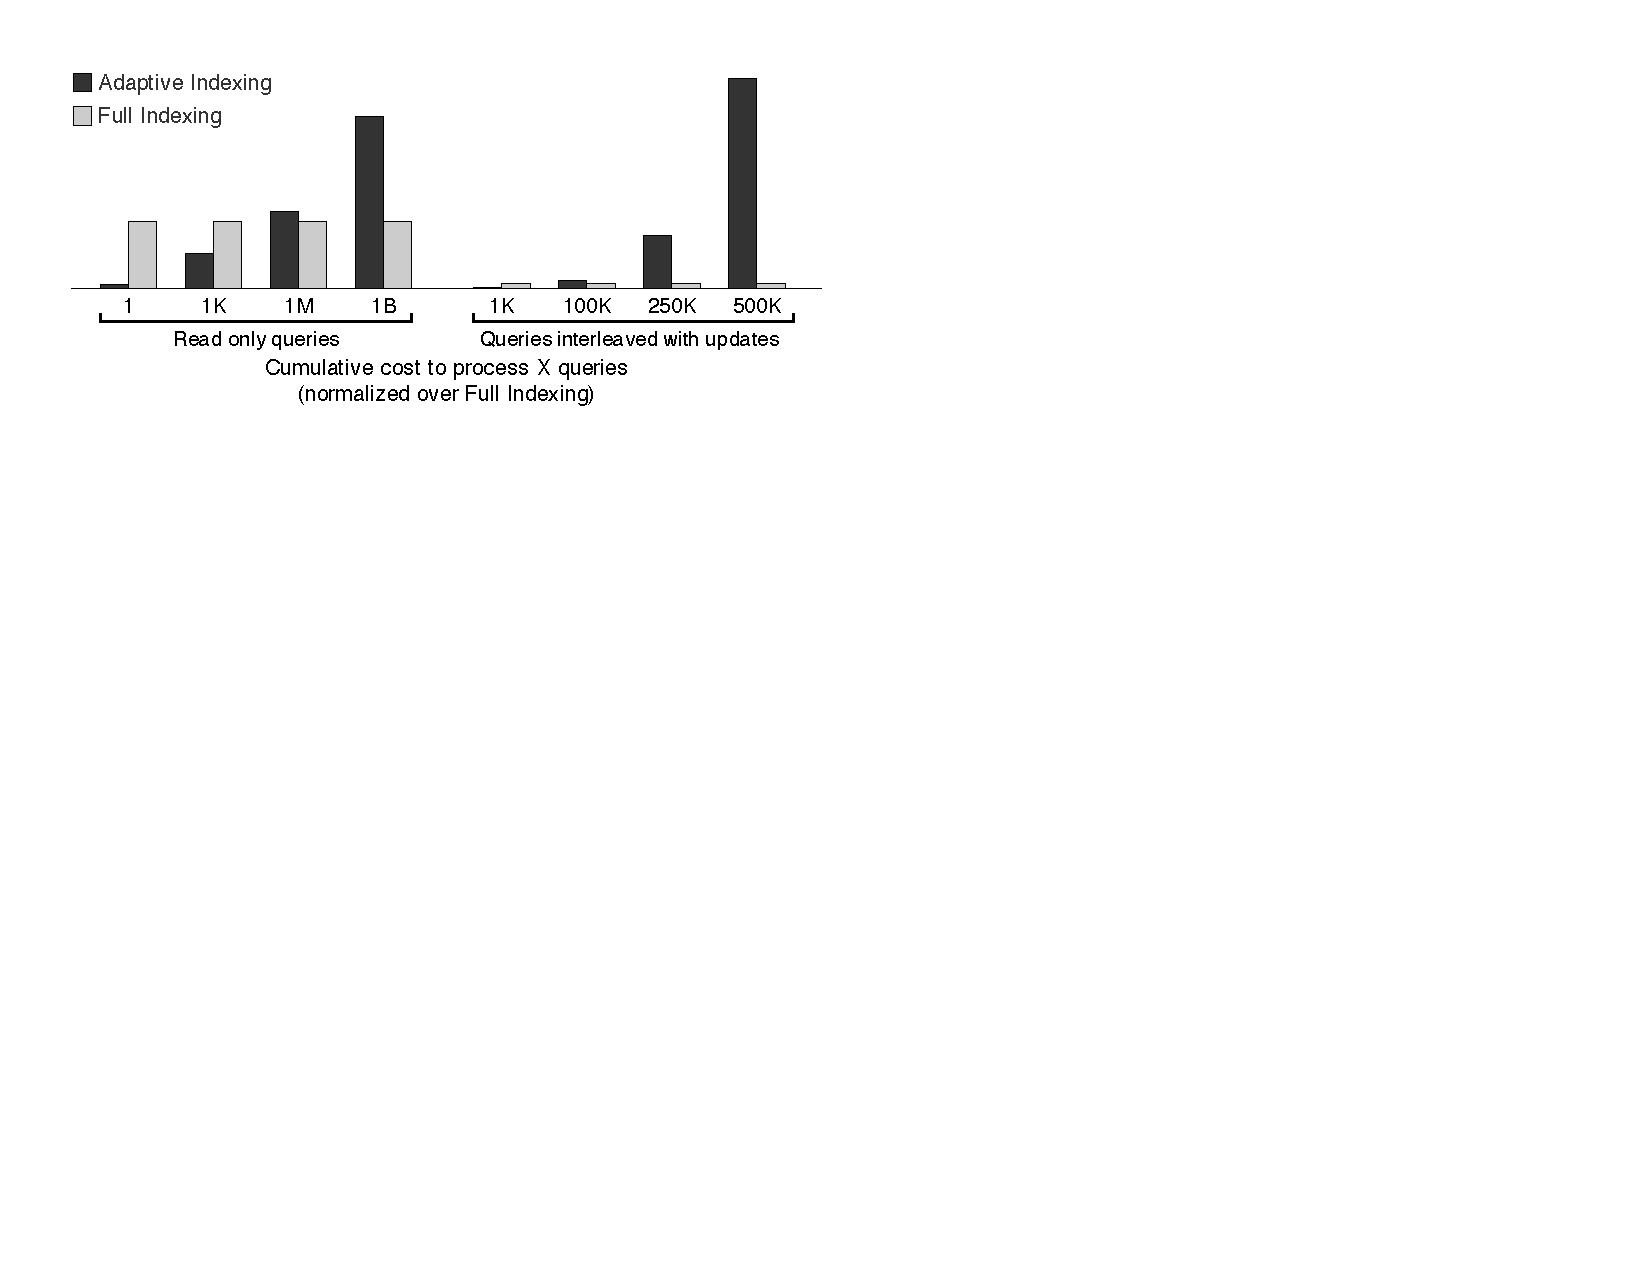
\includegraphics[width=0.85\columnwidth]{graphs/motivation.pdf}%
%\vspace{-1.5em}
\caption{The need for transitive indexing: A different design is best for different stages of a workload.}
%\vspace{-2.5em}
\label{F:Motivation}
\end{figure}

\textbf{The Problem: Read-write Intensive Workloads.}
In this paper, we address the need of modern applications to handle workloads which require both efficient read and efficient update
support in the same system. 
There is an increasing attention to this problem at various levels, e.g., 
in terms of database architectures with efforts such as SAP HANA \cite{Hana} and Hyper \cite{hyper} or also at the indexing level
with efforts such as ART main-memory indexing \cite{art}.
A problem with traditional  static indexing approaches is that one has to know exactly which data should be indexed
and then also have the time and resources to go through a very expensive indexing phase.
As applications become more and more real-time and with ad-hoc querying demands, such static approaches
become a bottleneck to having a quick access to new data.
A number of adaptive indexing approaches have been proposed lately to address exactly this problem of static indexing \cite{IKM:CIDR07,hail}.
With adaptive indexing, indexes are built and refined incrementally during query processing
by treating each query as an advice of how data should be stored.
However, we show that although existing adaptive indexing techniques 
do provide significant improvement for ad-hoc workloads, minimizing or even eliminating initialization costs, 
they are not resilient in the same way that non-adaptive indexing is for read-write intensive workloads. 

\textbf{Motivating Example.}
Figure \ref{F:Motivation} demonstrates this problem: it depicts the relative time needed ($y$-axis) 
to answer the first X queries ($x$-axis) in a long sequence of random range 
queries and updates over a single column of $10^8$ tuples (10 updates arrive every 10 read queries). 
Each graph is normalized (independently) over its static indexing costs.
In this case, for static indexing we use the state-of-the-art in memory index ART \cite{art}
while for adaptive indexing we use the state-of-the-art stochastic cracking index \cite{StochasticCracking}.
Figure \ref{F:Motivation} shows that while early in the query sequence adaptive indexing 
significantly outperforms static indexing,
as the sequence evolves,
adaptive indexing loses its advantage over static indexing, i.e.,  it is not resilient.
The first query for adaptive indexing is more than 10 times faster than static indexing;
Full indexing needs to fully index the column, while adaptive indexing performs only small index refinement actions with every query.
However, as more queries and updates arrive, adaptive indexing eventually becomes more than 10 times slower than static indexing.

Ideally, we would like to maintain the performance of adaptive indexing early in the query sequence 
and the performance of static indexing later on.


\textbf{Contributions: Transitive Indexing.}
Our contributions are as follows.
\begin{itemize}

\item We propose a new main-memory indexing research area, termed 
\emph{transitive indexing}.
The idea is that a data structure representing an index does not have a static shape.
Instead, its shape morphs over time as the workload evolves.

\item
We present Trimmer, a transitive indexing approach which  
initially requires no preparation or initialization steps.
Data is simply appended in the form of vectors with no order forced
both inside each vector and across vectors.
As the workload evolves, Trimmer starts forcing order and structure.
Each vector is independently indexed and refined, while data starts flowing from vector to vector.
Gradually, the vectors start morphing into a Trie structure optimized for main-memory.
Only the hot part of the data morphs and everything happens during query processing
without any need for any administration or control.

\item
We show that Trimmer  maintains all the good properties of 
both existing adaptive indexing approaches and those of non-adaptive approaches, 
i.e., it is lightweight, it continuously adapts by incrementally refining indexes
and it requires zero workload knowledge and preparation costs.
At the same time it is resilient, i.e., it maintains its performance advantages
unfettered even under long strings of queries and continuous data updates;
it is geared towards continuous on-the-fly data exploration under massive updates. 

\end{itemize}

We experimentally demonstrate the advantages of Trimmer
over existing static indexing and adaptive indexing techniques. 
We use both synthetic benchmarks as well as real world data and queries.
For example, in experiments with a 4 Terabyte instance of 
data and queries from the Sloan Digital Sky Survey/SkyServer
from the astronomy domain,
we show that Trimmer can handle a combined workload of $15*10^4$ queries and $5*10^8$ updates in roughly 1 minute, while 
state-of-the-art adaptive indexing needed more than 16 hours and state-of-the-art non adaptive indexing needs ??. 

%\textbf{Paper Organization.}
%The rest of the paper is organized as follows.
%Section \ref{sec:related} discusses background and related work.
%Then, Section \ref{sec:problem} presents in detail the resilience problem of 
%existing adaptive indexing techniques and their inability to cope with the requirements
%of continuous exploration.
%Section \ref{sec:cracke} presents a series of possible patches in existing adaptive indexing
%that deal with the problem only to a certain degree
%and then it introduces CTree for full resilient and adaptive exploration.
%In Section \ref{sec:experiments}, we present a detailed experimental analysis, demonstrating the effectiveness 
%and the advantages of CTree both on synthetic and on real workloads.
%Finally, Section \ref{sec:conclusion} discusses future work and concludes the paper.

%As we enter the era of data deluge one of the main emerging patterns is the need for
%data exploration techniques \cite{SurajitSigmod2012Keynote}.
%Data arrives continuously while businesses and sciences need to continuously pose
%queries in an adaptive and interactive mode \cite{NoDBcidr,Blinkmit,ResearcherGuide,Sciborg}.
%A characteristic property in such environments is that there is little idle time and workload knowledge. 
%
%\textbf{Physical Design.}
%Good performance in database systems largely relies on proper \emph{tuning} and \emph{physical design}.
%Typically, all tuning choices happen up-front, assuming sufficient workload knowledge
%and idle time. Workload knowledge is necessary in order to determine the appropriate
%tuning actions, while idle time is required in order to perform those actions.
%Modern database systems rely on auto-tuning tools to carry out these steps, e.g.,
%\cite{CN:VLDB:97,FST88,H76,SHU:VLDB:2004,DB2DesignAdvisor}.
%

%\textbf{Dynamic Environments.}
%However, in dynamic environments, workload knowledge and idle time are scarce resources.
%For example, in scientific databases new data arrive on a daily or even hourly basis,
%while query patterns follow an exploratory path as the scientists try to interpret the data
%and understand the patterns observed; there is no time and knowledge
%to analyze and prepare a different physical design hour-by-hour or even day-by-day.
%
%Traditional indexing via tuning presents three fundamental weaknesses in such cases:
%(a) the workload may have changed by the time we finish tuning;
%(b) there may be no time to finish tuning properly;
%and (c) there is no indexing support during tuning.
%
%\textbf{Adaptive Indexing.}
%Recently, a new approach to the physical design problem was proposed,
%namely \emph{database cracking} \cite{IKM:CIDR07}. %\cite{CrackingThesis}.
%Cracking introduces the notion of continuous, incremental, partial and on-demand adaptive indexing.
%Thereby, indexes are incrementally built and refined during query processing.
%Data is physically reorganized in a continuous manner, aiming to
%match the workload, by treating each query as an advice of how data should be stored.
%
%
%\textbf{The Problem. Non-Resilient Exploration.}
%At a first glance it would seem that existing adaptive indexing approaches can cover the need
%towards adaptive exploration in the era of data deluge. 
%However, in this paper we show that 
%existing adaptive indexing techniques such as database cracking, adaptive merging and their variations
%do not cope with these new challenges. The fundamental weaknesses we identify are the inability to 
%support long strings of exploratory queries interleaved with  updates.
%Figure \ref{F:Motivation} demonstrates this problem: it depicts the relative time needed ($y$-axis) 
%to answer the first X queries ($x$-axis) in a long sequence of random select 
%queries and updates over a single column of $10^8$ tuples. 
%Each graph is normalized (independently) over its full indexing costs.
%Figure \ref{F:Motivation} shows that as the sequence evolves in the read only case,
%adaptive indexing (cracking) loses its advantage over a traditional full indexing approach, i.e.,  it is not resilient.
%The first query for cracking is more than 10 times faster than full indexing;
%Full indexing needs to fully index the column, while cracking performs only small index refinement actions with every query.
%However, as more queries arrive, cracking eventually becomes 2 times slower than full indexing.
%The performance degradation is significantly worse when continuous updates interleave with read queries
%(10 updates arrive every 10 read queries).
%In order to cope with the data deluge, 
%we would like to keep both the lightweight and the adaptive behavior of cracking for the early queries,
%while still maintaining this behavior in the long run even during continuous updates. 
%
%
%\textbf{The Solution. Comb: Resilient Adaptive Indexing.}
%In this paper, we propose a new adaptive indexing approach, termed 
%\emph{ Comb (Cracking Over Malleable Buckets)}.
%Comb maintains all the good properties of existing 
%approaches, i.e., it is lightweight, it continuously adapts by incrementally refining indexes
%and it requires zero workload knowledge and preparation costs.
%At the same time it is resilient, i.e, it maintains its performance advantages
%unfettered even under long strings of queries and continuous data updates;
%it is geared towards on-the-fly data exploration. 
%
%Comb is designed for main memory column-stores; it breaks a single column into multiple disjoint pieces
%and each piece is indexed, accessed and updated independently, while data flows from piece to piece in an adaptive way
%when the index needs to be balanced. 
%We present Comb in detail and we experimentally demonstrate its advantages
%over existing indexing and adaptive indexing techniques. 
%We use both synthetic benchmarks as well as real world data and queries.
%For example, in experiments with a 4 Terabyte instance of 
%data and queries from the Sloan Digital Sky Survey/SkyServer
%from the astronomy domain,
%we show that Comb can handle a combined workload of $15*10^4$ queries and $5*10^8$ insertions in roughly 1 minute, while 
%state-of-the-art adaptive indexing needed more than 16 hours. 
%
%\textbf{Paper Organization.}
%The rest of the paper is organized as follows.
%Section \ref{sec:related} discusses background and related work.
%Then, Section \ref{sec:problem} presents in detail the resilience problem of 
%existing adaptive indexing techniques and their inability to cope with the requirements
%of continuous exploration.
%Section \ref{sec:cracke} presents a series of possible patches in existing adaptive indexing
%that deal with the problem only to a certain degree
%and then it introduces Comb for full resilient and adaptive exploration.
%In Section \ref{sec:experiments}, we present a detailed experimental analysis, demonstrating the effectiveness 
%and the advantages of Comb both on synthetic and on real workloads.
%Finally, Section \ref{sec:conclusion} discusses future work and concludes the paper.
%






%\section{Related work}
\label{sec:related}

In this section, we provide the necessary background and discuss related work.
We briefly recap the three approaches to indexing and tuning, i.e.,
offline analysis, online analysis, and adaptive indexing.


\textbf{Offline Analysis.}
Offline analysis or {\em auto-tuning} tools exist
in every major database product. They rely on the what-if analysis
paradigm and close interaction with the system's query optimizer
\cite{CN:VLDB:97,FST88,H76,SHU:VLDB:2004,DB2DesignAdvisor}.
Such approaches are non-adaptive: they render index tuning distinct from query processing operations.
They first monitor a running workload
and then decide what indexes to create or drop based on the observed patterns.
Once a decision is made, it affects all key ranges in an index, while index tuning and
creation costs impact the database workload as well.
Unfortunately, one may not have sufficient workload knowledge
and/or idle time to invest in offline analysis in the first place.
Furthermore, with dynamic workloads, any offline decision
may soon become invalid.

% better connect with preceding paragraph
\textbf{Online Analysis.}
Online analysis aims to tackle the problem posed by such dynamic workloads.
A number of recent efforts attempt to provide viable online indexing solutions
\cite{OnlineTuning, Colt, Tune, LSSS07}.
Their main common idea is to apply the basic concepts of offline analysis online:
the system monitors its workload and performance while processing queries,
probes the need for different indexes and, once certain thresholds are passed, triggers
the creation of such new indexes and possibly drops old ones.
However, online analysis may severely overload individual query processing during index creation.
Approaches such as soft indexes \cite{LSSS07} try to exploit
the scan of relevant data (e.g., by a select operator) and send this data to a full-index creation routine at the same time. This way, data to be indexed is read only once.
Still, the problem remains that creating {\em full} indexes significantly penalizes individual queries.

% some editing here, just to avoid self-plagiarism and some repetitions
\textbf{Database Cracking.}
The drawbacks of offline and online analysis motivate {\em adaptive indexing},
the prime example of which is {\em database cracking} \cite{CrackingThesis}.
Database cracking pioneered the notion of continuously and incrementally building and refining
indexes as part of query processing;
it enables efficient adaptive indexing, where index creation and optimization
occur collaterally to query execution;
thus, only those tables, columns, and key ranges that are queried are being optimized.
The more often a key range is queried, the more its representation is refined.
Non-queried columns remain non-indexed, and non-queried key ranges are not optimized.

\begin{figure}[t]
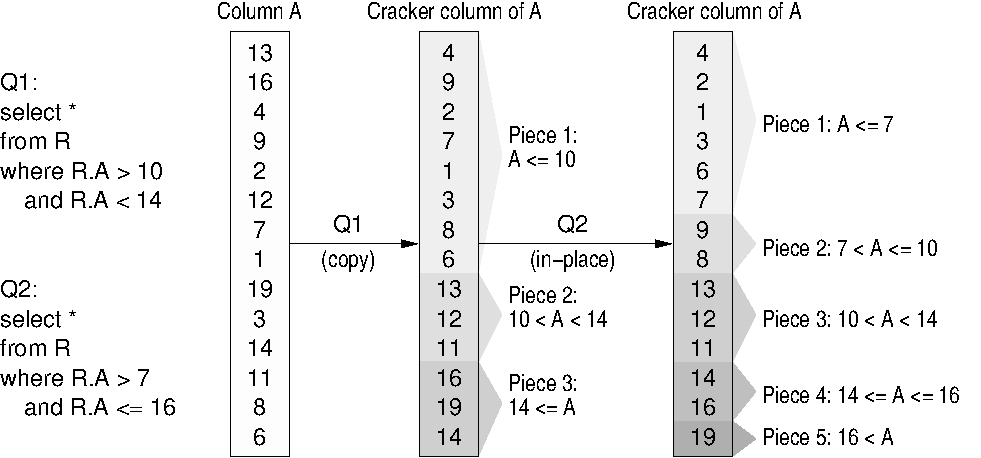
\includegraphics[width=.95\columnwidth]{CrackExample.pdf}
\vspace{-1em}
\caption{Cracking a column.}
\vspace{-2em}
\label{F:CrackExample}
\end{figure}

\textbf{Selection Cracking.}
We now briefly recap \emph{selection cracking} \cite{IKM:CIDR07}.
The main innovation is that the physical
data store is continuously changing with each incoming query $q$, using $q$
\emph{as a hint on how data should be stored}.
Assume a query requests $A$$<$$10$.
In response, a cracking DBMS clusters all tuples of $A$ with
$A$$<$$10$ at the beginning of the respective column $C$,
while pushing all tuples with $A$$\geq$$10$ to the end.
A subsequent query requesting $A$$\geq$$v_1$, where $v_1$$\geq$$10$,
has to search and crack only the last part of $C$ where values $A$$\geq$$10$ reside.
Likewise, a query that requests $A$$<$$v_2$, where $v_2$$\leq$$10$,
searches and cracks only the first part of $C$.
All crack actions happen as part of the query operators, requiring no external administration.
Figure~\ref{F:CrackExample} shows an example of two queries cracking a column
using their selection predicates as the partitioning bounds. Query Q1 cuts the column
in three pieces and then Q2 enhances this partitioning more by cutting the first and
the last piece even further, where its low and high bound fall.
Each query collects its qualifying tuples in a contiguous area.

%The terminology ``cracking" reflects the fact that
%the database is partitioned (cracked) into smaller and manageable pieces.

Cracking gradually improves data access, eventually leading to a significant speed-up in query
processing \cite{IKM:CIDR07,IKM:SIGMOD09}, even during updates \cite{IKM:SIGMOD07};
%
% we have to explain this happens because we are in a column-store
as it is designed over a column-store it is applied at the attribute level; a query results in reorganizing the
referenced column(s), not the complete table;
it is propagated across multiple columns on demand,
depending on query needs with \emph{partial sideways cracking} \cite{IKM:SIGMOD09}, whereby
pieces of cracker columns are dynamically created and deleted based on storage restrictions.
In \cite{Concurrency}, the authors show how to enable concurrent queries via limited concurrency control effort, 
relying purely on latches as cracking read queries change only the index structure while the index contents remain intact.
In addition, stochastic cracking \cite{StochasticCracking} 
performs non-deterministic cracking actions by following query bounds less strictly. This way it allows for a more even spread of the partitioning across a column, preventing the lingering of large unindexed areas that are expensive to crack in the future.



\emph{Adaptive merging} \cite{GK10a,GK10b}, extends cracking
to adopt a partition/merge\hyp{}like logic with active sorting steps;
while original cracking can be seen as an incremental quicksort,
adaptive merging can be seen as an incremental external merge sort.

More recently, \cite{AdaptiveIndexing} studied the broader space of adaptive indexing;
it combines insights from both cracking \cite{IKM:CIDR07} and adaptive merging \cite{GK10a,GK10b},
to devise adaptive indexing algorithms (from very active to very lazy) that improve over both these predecessors.
%
%it exploits a partition/merge -like logic as well, to design a broad collection of very active
%to very lazy adaptive algorithms; it improves over both original cracking and adaptive merging.

%The key benefit of database cracking is its lightweight nature:
%the overhead for incremental index creation is minimal,
%and disappears once a range has been fully optimized.
The benchmark proposed in \cite{GIKM10} discusses
the requirements for adaptive indexing;
(a) lightweight initialization, i.e., low cost for the first few queries
that trigger adaptation; and (b) as fast as possible convergence to the desired performance.
%Low cost is measured against the default approach of a full scan, while
%desired/optimal performance is measured against the performance of a full index.
Initialization cost is measured against that of a full scan, while
desired performance is measured against that of a full index.
A good adaptive indexing technique should strike a balance between those
two conflicting parameters \cite{GIKM10,AdaptiveIndexing}.
We follow these guidelines in this paper as well.


% use \hyp{} for problem-less hyphenation with line splitting
To date, all work on cracking and adaptive indexing has focused on main memory environments;
%in these environments,
persistent data may be on disk but the working data set for a given query (operator in a column-store)
should fit in memory for efficient query processing.
In addition, the partition/merge\hyp{}like logic introduced in \cite{AdaptiveIndexing,GK10a,GK10b}
can be exploited for external cracking. %(disk-based) cracking.
%As we show, stochastic cracking applies with this partition/merge -like logic as well.
% no need, mentioned below


The basic underlying physical reorganization routines remain unchanged in all existing adaptive indexing work;
therefore, for ease of presentation, we initially discuss our work 
building on top of the original cracking technique \cite{IKM:CIDR07}.
In Section \ref{sec:experiments}, we show that the resilience problem occurs in all adaptive indexing approaches
and that our new indexing technique, Comb, enjoys a significant advantage over all of them.


\textbf{Column-Stores.}
Database cracking and all adaptive indexing studies so far rely on a number of modern column-store design characteristics.
Column-stores store data one column at a time in fixed-width dense arrays
\cite{manegold00, stonebreaker05vldb, X100}.
This representation is the same both on disk and in memory and allows for efficient
physical reorganization of arrays.
%In contrast, if data representation was variable width
%then moving data around would be significantly more expensive as we would also have to make sure
%there is enough free space in the new position as well as update and maintain the proper
%metadata.
Similarly, column-stores rely on bulk and vector-wise processing.
Thus, a select operator typically processes a single column in vector format at once,
instead of whole tuples one at a time.
In effect, cracking performs all physical reorganization actions
efficiently in one go over a column. For example, the cracking select operator physically
reorganizes the proper pieces of a column to bring all qualifying values in a contiguous area
and then returns a view of this area as the result.

%
\section{The Problem}
\label{sec:problem}

In this section, we motivate the need for resilient adaptive indexing in modern applications.
We first demonstrate the main advantages that existing adaptive indexing
techniques bring and then we highlight the core non-resilience problems that appear
when dealing with long strings of exploratory queries and continuous updates.
We use the original database cracking technique to highlight these benefits
and shortcomings of adaptive indexing. In Section \ref{sec:experiments},
we show that the same properties are still true for more complex adaptive indexing techniques
that were introduced more recently such as 
stochastic cracking \cite{StochasticCracking}, adaptive merging \cite{GK10b}  
and hybrid adaptive indexing \cite{AdaptiveIndexing}.


\subsection{Adaptive Behavior}
The main power of original database cracking is its ability to self-organize
automatically and at low cost.

The former feature (automatic self-organization) is crucial because it eschews the need for special decision-making as to when
the system should perform self-organizing actions;
the system self-organizes \emph{continuously} by default.
Apart from conferring benefits of efficiency and hands-free convenience in workload analysis,
such automatic self-organization also brings instant, online adaptation in response to a changing workload,
without delays.
In effect, there is no performance penalty due to having an unsuitable physical design
for a prolonged time period.

The latter feature (low cost) is also a powerful property that sets cracking apart
from approaches such as online indexing. This derives
from the ability to provide incremental and partial indexing integrated in an efficient way
\emph{inside} the database kernel.

\begin{figure}[t]
\hspace{-1em}
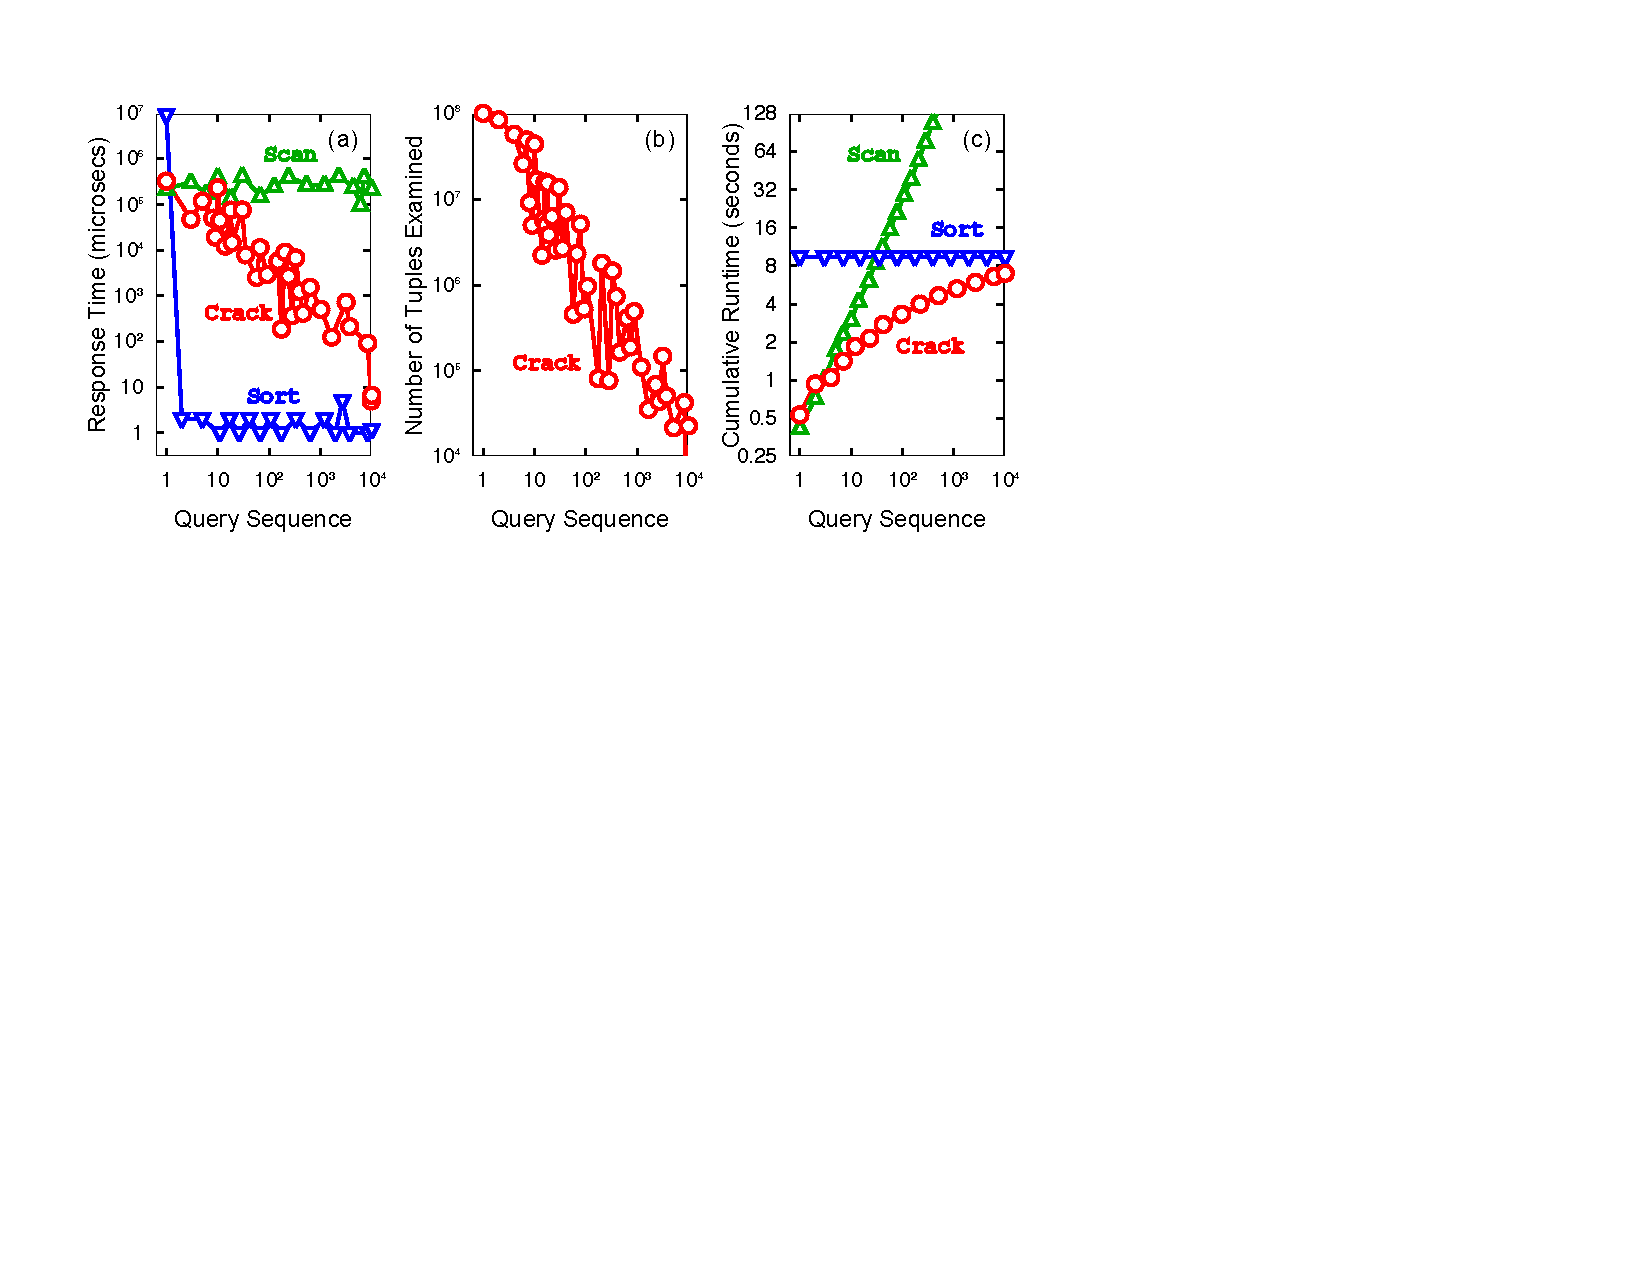
\includegraphics[width=1.05\columnwidth]{graphs/figure2.pdf}%
\vspace{-1em}
\caption{Adaptive behavior benefits of adaptive indexing.}
\vspace{-2em}
\label{F:BasicPerQuery}
\end{figure}

\textbf{Cracking Continuous Adaptation.}
As we have seen in the example of Figure \ref{F:CrackExample},
cracking feeds from the select operator, using the selection predicates to drive the way data is stored.
This way, after each query, data is clustered in a way such that the qualifying values for the
respective select operator are in a contiguous area in the attribute column. 
The more queries are processed, the more knowledge and structure
are introduced; this is how cracking achieves instant adaptation.



\textbf{Cracking Cost.}
Let us now discuss the cost of cracking, i.e., the cost to run the select operator, which includes the cost
for identifying what kind of physical reorganizations are needed and performing such reorganizations.

A cracking DBMS maintains indexes, showing which piece of the array holds which value range,
in a tree structure; original cracking uses AVL-trees \cite{IKM:CIDR07}.
Thus the cost of a query is the cost to search the tree in order to determine
the portion of the array which needs to be cracked plus the cost to perform the actual data reorganization.
For example, in Figure \ref{F:CrackExample} $Q1$ needs to analyze all tuples in the column
in order to achieve the initial clustering, as there is no prior knowledge about the structure of the data.
The second query, $Q2$, can exploit the knowledge gained by $Q1$ and avoid touching part of the data.
With $Q1$ having already clustered the data into three pieces, $Q2$ needs to touch only
two of those, namely the first and third piece. That is because the second piece created by $Q1$
already qualifies for $Q2$ as well.

Generalizing the above analysis, we infer that, assuming such range queries (select operators),
a query will analyze as most two \emph{end} pieces, i.e., the ones intersecting with the query's requested value range boundaries.
As more pieces are created by every query that does not find an exact
match, pieces become smaller.

\begin{figure*}[t]
\hspace{6.5em}%
\Fig[b]{1\columnwidth}{%
\hspace{-6.5em}%
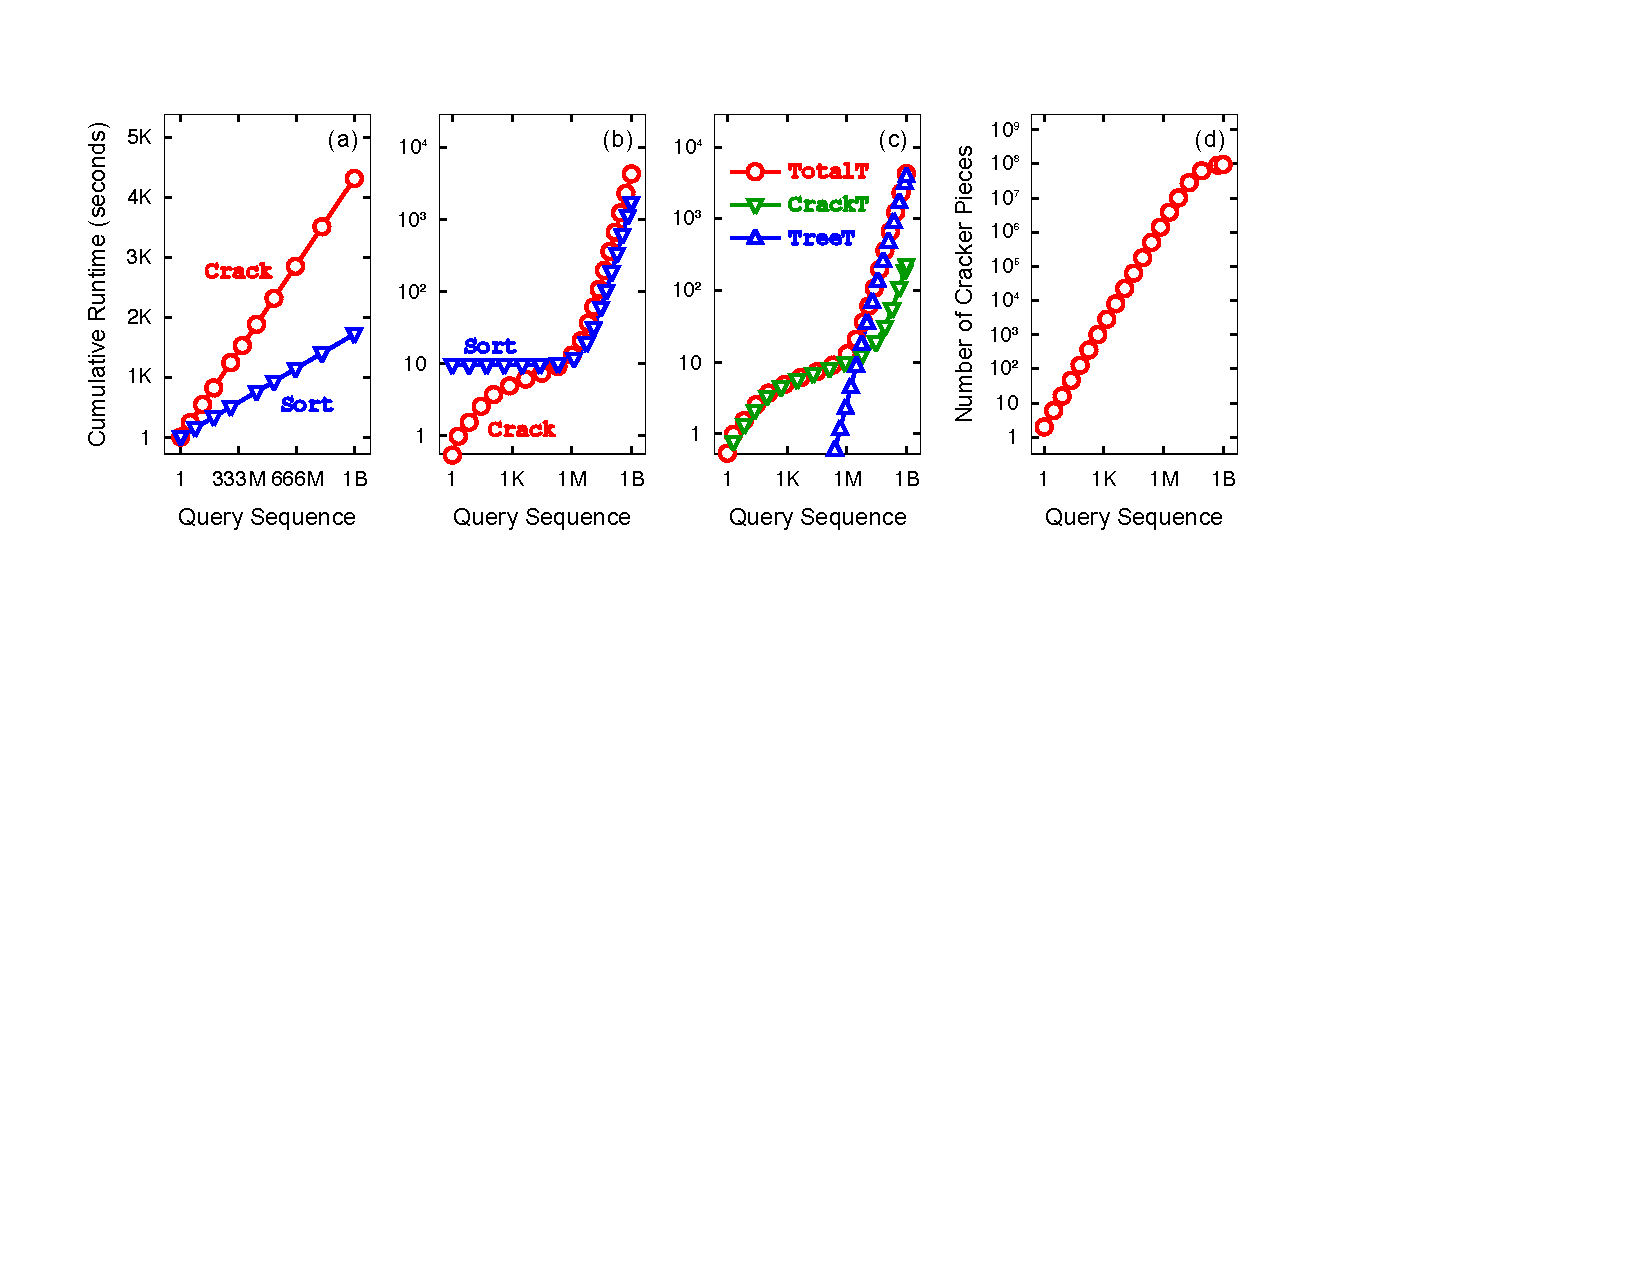
\includegraphics[width=1.5\columnwidth]{graphs/figure3.pdf}
\vspace{-2.5em}
\caption{Non-resilience during long query sequences.}
\vspace{-2em}
\label{F:LongSequenceProblem}
}
\hfill
\hspace{6.5em}%
\Fig[b]{.6\columnwidth}{%
\hspace{1.5em}%
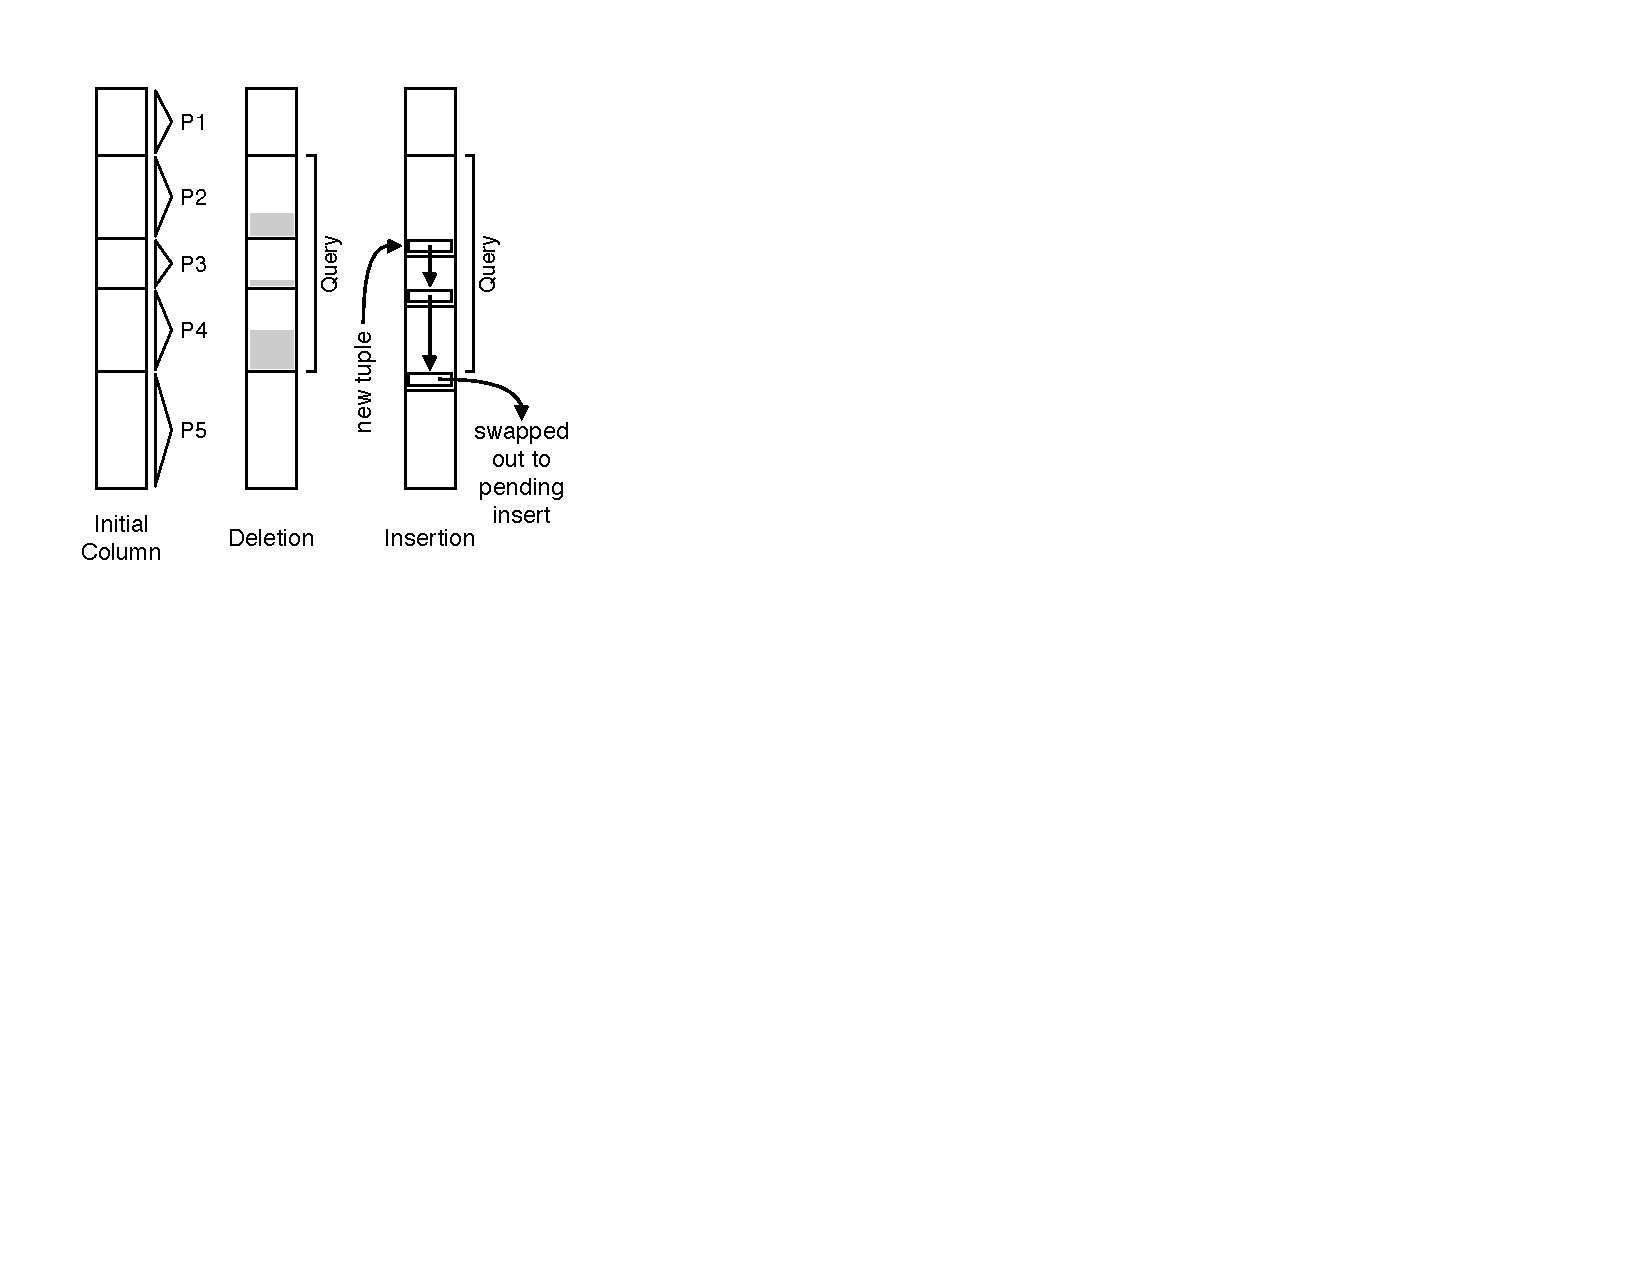
\includegraphics[width=.9\columnwidth]{graphs/fig_mrd_mri.pdf}%
\vspace{-1em}
\caption{Database cracking updates.}
\vspace{-2em}
\label{F:updates}
}
\end{figure*}


\textbf{Basic Cracking Performance.}
Figure \ref{F:BasicPerQuery}(a) shows a performance example where cracking is compared against
a full indexing approach ({\sf Sort}), in which we completely sort the column with the first query.
In an in-memory column-store, sorting a column creates the perfect index which allows for very fast
data access using binary search given that the underlying storage is 
fixed-width and dense arrays.
The data for this experiment consists of $10^8$ tuples of unique integers in $[0,2^{31})$.
The query workload is random -- the bounds are random while 
the ranges requested have a fixed selectivity of 1\% per query.
This scenario assumes a dynamic environment where there is no workload knowledge or idle time
in order to pre-sort the data, i.e., our very motivating example for adaptive indexing.


As Figure \ref{F:BasicPerQuery}(a) shows, once the data is sorted with the first query, from then on performance is
extremely fast as we only need to perform a binary search over the sorted column to satisfy each select operator request.
Nevertheless, the problem is that we overload the first query. On the other hand, database cracking
continuously improves performance without penalizing individual queries. Eventually, its performance reaches
the levels of {\sf Sort}.\
The benefit of cracking comes by continuously analyzing less and less data.
Figure \ref{F:BasicPerQuery}(b) shows the number of tuples each cracking query has to touch;
as we process more queries, more pieces are created by cracking the column and subsequent queries can 
reduce the amount of data touched by exploiting the more fine-grained index.

We also compare against a plain {\sf Scan} approach where data is always completely scanned. 
Naturally, as Figure \ref{F:BasicPerQuery}(a) shows, this has a stable behavior;
we observe that cracking does not significantly penalize any query more than the default {\sf Scan} approach.
Note, that while cracking and {\sf Sort} can simply return a view of the (contiguous)
qualifying tuples, {\sf Scan} has to materialize
a new array with the result. 

Figure \ref{F:BasicPerQuery}(c) shows the same results as in Figure \ref{F:BasicPerQuery}(a) but uses
a different metric; this time the graph plots the cumulative time as the query sequence evolves, i.e.,
every point $(x,y)$ depicts that it takes $y$ seconds in total to process the first $x$ queries.
Remarkably,  by the time cracking has already answered all $10^4$ queries
the full indexing approach still has not finished preparing the index. 
In dynamic environments with little idle time to invest in index preparation and with little knowledge
about which columns are actually interesting for the queries, adaptive indexing has a huge advantage.
Full offline indexing has no time to prepare and no intelligence  about which columns to index.
In the specific example in our experiment, if the workload changes sometime during those $10^4$ queries,
then full indexing is simply a waste of resources. 


\subsection{Problem 1: Long Query Sequences}
The previous discussion highlighted the main motivation and benefits of adaptive indexing.
Here, we expose the non-resilience problem when it comes to long exploratory query sequences.
We use a similar experiment as before with the same set-up;
the difference is that now we fire a significantly longer query sequence, i.e., up to 1 
billion queries as opposed to only $10^4$  queries we had before.

Figure \ref{F:LongSequenceProblem} shows the results, comparing cracking to full sorting.
Figure \ref{F:LongSequenceProblem}(a) depicts the cumulative response time.
It reveals that as the query sequence evolves, cracking loses its advantage over full sorting. 
The total cost for cracking at the end of the query sequence is more than 4000 seconds while 
full sorting needed less than half of that. The advantage of cracking early in the query sequence still remains. 
Figure \ref{F:LongSequenceProblem}(b) shows the same results with 
a log scale for both axes.
Up to roughly 1 million queries cracking enjoys a better performance. 
However, after this point, we reach a threshold where it would have been better to not use adaptive indexing
when considering the cumulative costs for the whole query sequence.

We analyze this behavior further by breaking down the cracking costs
in Figures \ref{F:LongSequenceProblem}(c) and (d). 
Figure \ref{F:LongSequenceProblem}(c) shows the total cracking costs (TotalT)
separated into the costs of searching the tree of the cracking index (TreeT) and to the cost of performing the actual cracking (CrackT),
i.e., the actual physical reorganization of the column. 
The cumulative time of these break-down metrics 
as the sequence evolves shows that
up to the threshold of 1 million queries the total query cost is dominated by the cracking costs of reorganizing the column.
However, after this point the cost is dominated by the cost of searching the tree.
Figure \ref{F:LongSequenceProblem}(d) verifies that searching the tree becomes the main bottleneck;
it plots the number of pieces in the cracking index. As we pose more queries, more pieces are created (at most 2 pieces per query)
and hence the tree grows and becomes more expensive to search due to random access.



\subsection{Problem 2: Continuous Data Updates}

Having seen the problem with long query sequences, we highlight 
an even more significant source of non-resilience
with existing adaptive indexing -- performance degradation in long sequences where 
updates interleave with queries.

\textbf{Cracking Updates.}
Let us first give a short description of how cracking performs updates as  proposed in \cite{IKM:SIGMOD07}.
To deal with updates, original cracking uses an adaptive approach. Updates (inserts or deletes)
are marked as pending updates upon arrival. For each column, there is a pending insertions and a pending deletions column.
Thus, update queries are  close to zero-cost queries as they do nothing more than appending the new updates at
the pending columns.
When read queries arrive, they on-the-fly merge any pending updates in the actual cracking columns.
They do so only for the updates that fall within the value range requested by the current query, enhancing the adaptive
behavior of cracking. If a range is never queried, then it is never updated.
The select operator is now responsible for both cracking and merging any qualifying updates at the proper cracking
pieces.
The merge actions do not destroy the cracker index, i.e., all the partitioning information is maintained.
Given that original cracking works on top of fixed-width and dense columns, it needs to ripple/shuffle values 
such that it can place new values in the proper pieces.
Figure \ref{F:updates} shows an example of how tuples need to be moved across pieces when inserting 
a new tuple or when removing an existing one.
Given that within each cracking piece values are not ordered, not all values within a piece need to be moved;
to move a full piece one position down, it is sufficient to move the first value of the piece to the end of this piece
and subsequently change the borders of the piece.
Deletes leave back holes, while a select operator makes sure that it ripples all holes at the borders of the piece
where they belong so that subsequent operators on this range can more easily go through the tuples of this piece. 
Holes are exploited to place new tuples in when possible.


\textbf{The Problem.}
To demonstrate the non-resilience problem in long sequences where
updates interleave with queries, 
we perform the same experiment as before; the difference now is that data is not static anymore.
Now data arrival events interleave with queries.
This scenario matches modern applications where data arrive periodically  but quite often, i.e., 
every few hours or minutes, while we still want to explore the data for interesting patterns in online manner.
The set-up is the same as in the previous experiment;
the difference here is that every  10 read queries, 10 random insert queries and 10 random delete queries arrive.

Figure \ref{F:UpdatesProblem} shows the results for cracking as the query sequence evolves.
Figure \ref{F:UpdatesProblem}(a) shows that after about $10^4$ queries the 
cumulative total cost (TotalT) grows significantly. 
Figure \ref{F:UpdatesProblem}(a) also breaks this cost down to the cost that each query spends
to merge any updates (InsertT), to merge any deletes (DeleteT) and to the actual cracking cost to reorganize the 
column (CrackT). After $10^4$ queries the cost to merge the insertions becomes the dominant component and overshadows
the cracking costs by two orders of magnitude.
Figure \ref{F:UpdatesProblem}(b) depicts the amount of tuples examined as the query sequence evolves 
and the kind of actions performed. 
It shows that as we process more queries, significantly more tuples need to be touched.
In particular, significantly more tuples need to be rippled, i.e., they need to be moved into a new position
in the column. After $10^4$ queries, it is this action that dominates the actions performed and thus the total cost.
As more pieces are created, more data movement is needed in order to maintain
the partitioning information in the index. In this way, as the sequence evolves, performance degrades
due to the excessive update and administration costs.

Comparing Figure \ref{F:UpdatesProblem}(a) to 
Figure \ref{F:LongSequenceProblem}(b) (where we had no updates), we see that the performance
degradation occurs much earlier when updates interleave with queries, 
i.e., after only $10^4$ queries versus after $10^6$ queries in the read only scenario. 







%\begin{figure}[t]
\center
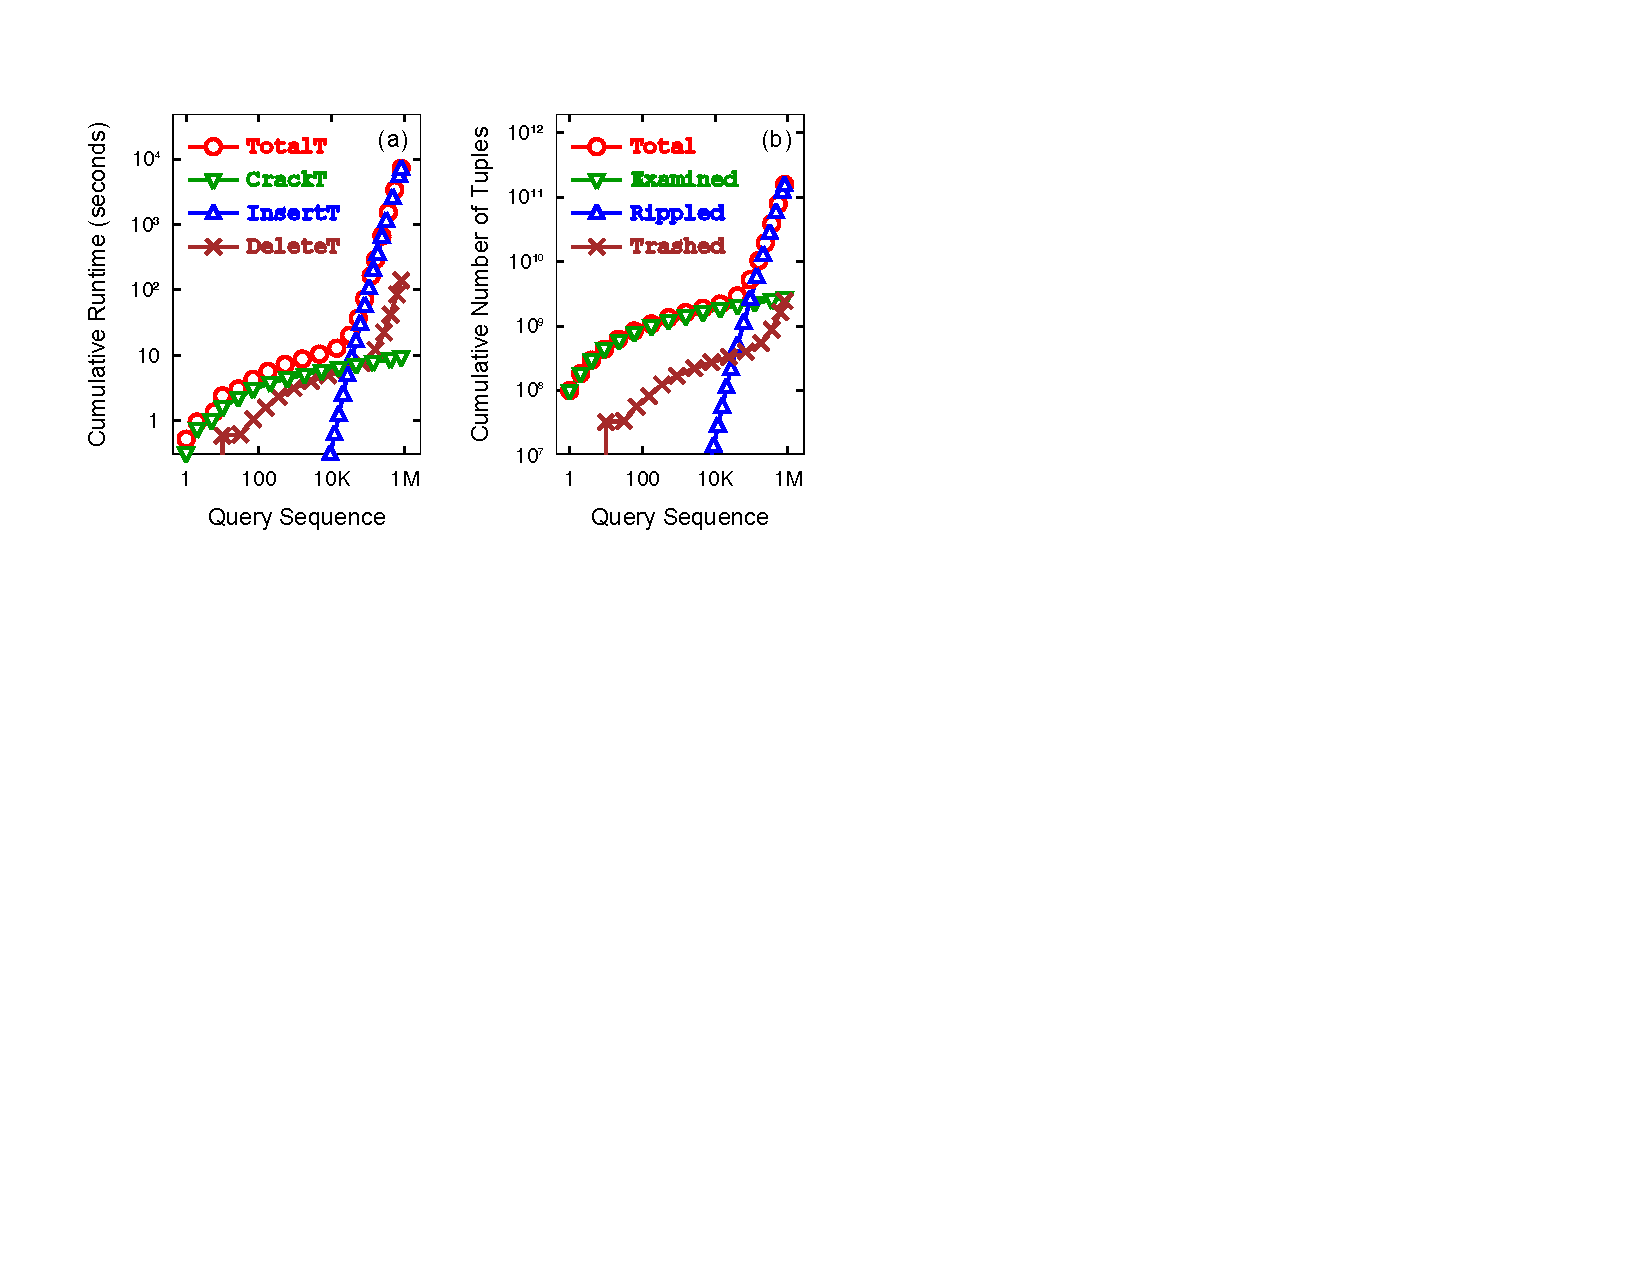
\includegraphics[width=.9\columnwidth]{graphs/figure4.pdf}
\vspace{-1em}
\caption{Non-resilience of adaptive indexing during long sequences of data injections interleaved with queries.}
\vspace{-1em}
\label{F:UpdatesProblem}
\end{figure}
\section{Resilient Adaptive Indexing}
\label{sec:cracke}

We showed in the previous section that while current adaptive indexing brings some significant advantages,
when it comes to long exploratory query sequences, especially when those are interleaved with updates,
then adaptive indexing loses all its performance advantages.
To deal with modern exploratory applications, we need adaptive indexing techniques which are resilient
to such problems and can maintain their adaptive properties in the long term.
In this section, we study the space of possible solutions and we propose Comb (Cracking Over Malleable Buckets), a new 
adaptive indexing technique that maintains all the desirable properties of current approaches,
while it is also resilient to cope with the data deluge challenges. 


\subsection{Target Performance}

Our goal is to maintain the main properties of existing adaptive indexing techniques
both {\em early} in a query sequence and as the query sequence {\em evolves}.
In this way, our target performance includes the following characteristics.
\begin{itemize}
\item \textbf{Lightweight}. The per query cost should be kept low, i.e., individual queries should not be penalized.
\vspace{-.5em}%
\item \textbf{Adaptive}. The system should be able to rapidly adjust to workload patterns.
\vspace{-.5em}%
\item \textbf{Resilient}. Performance should not degrade in the long run and all adaptive properties should be maintained.
\end{itemize}

\subsection{The Source of the Problem}

We can attribute the non-resilience problem of existing adaptive indexing techniques to
the maintenance and handling costs of the growing index structure
and of the dense array data structures.
As we have shown in Section \ref{sec:problem}, as query sequences evolve, 
the information stored in the index grows and it becomes much harder to maintain and traverse. 
The tree structure holding information regarding value ranges and piece boundaries grows with every 
query that  refines the index. Thus, as the query sequence grows, the tree grows as well and its traversal
leads to random memory access. In addition, in order to maintain the dense structure  of columns
and the partitioning information, 
merging of updates results in tuples being shuffled around.
The more the pieces in a cracking column, i.e., the more the information in the index, the more tuple
movements we have to do in order to put new values in or in order to move holes caused by deletions outside a given range.  

In order to deal with the non-resilience problem, we need to contain these extra costs, i.e., allow for
less expensive traversal of the tree part of the index and more efficient merging of updates.

\begin{figure*}[t]
\hspace{-3.5em}%
\Fig[b]{.5\columnwidth}{%
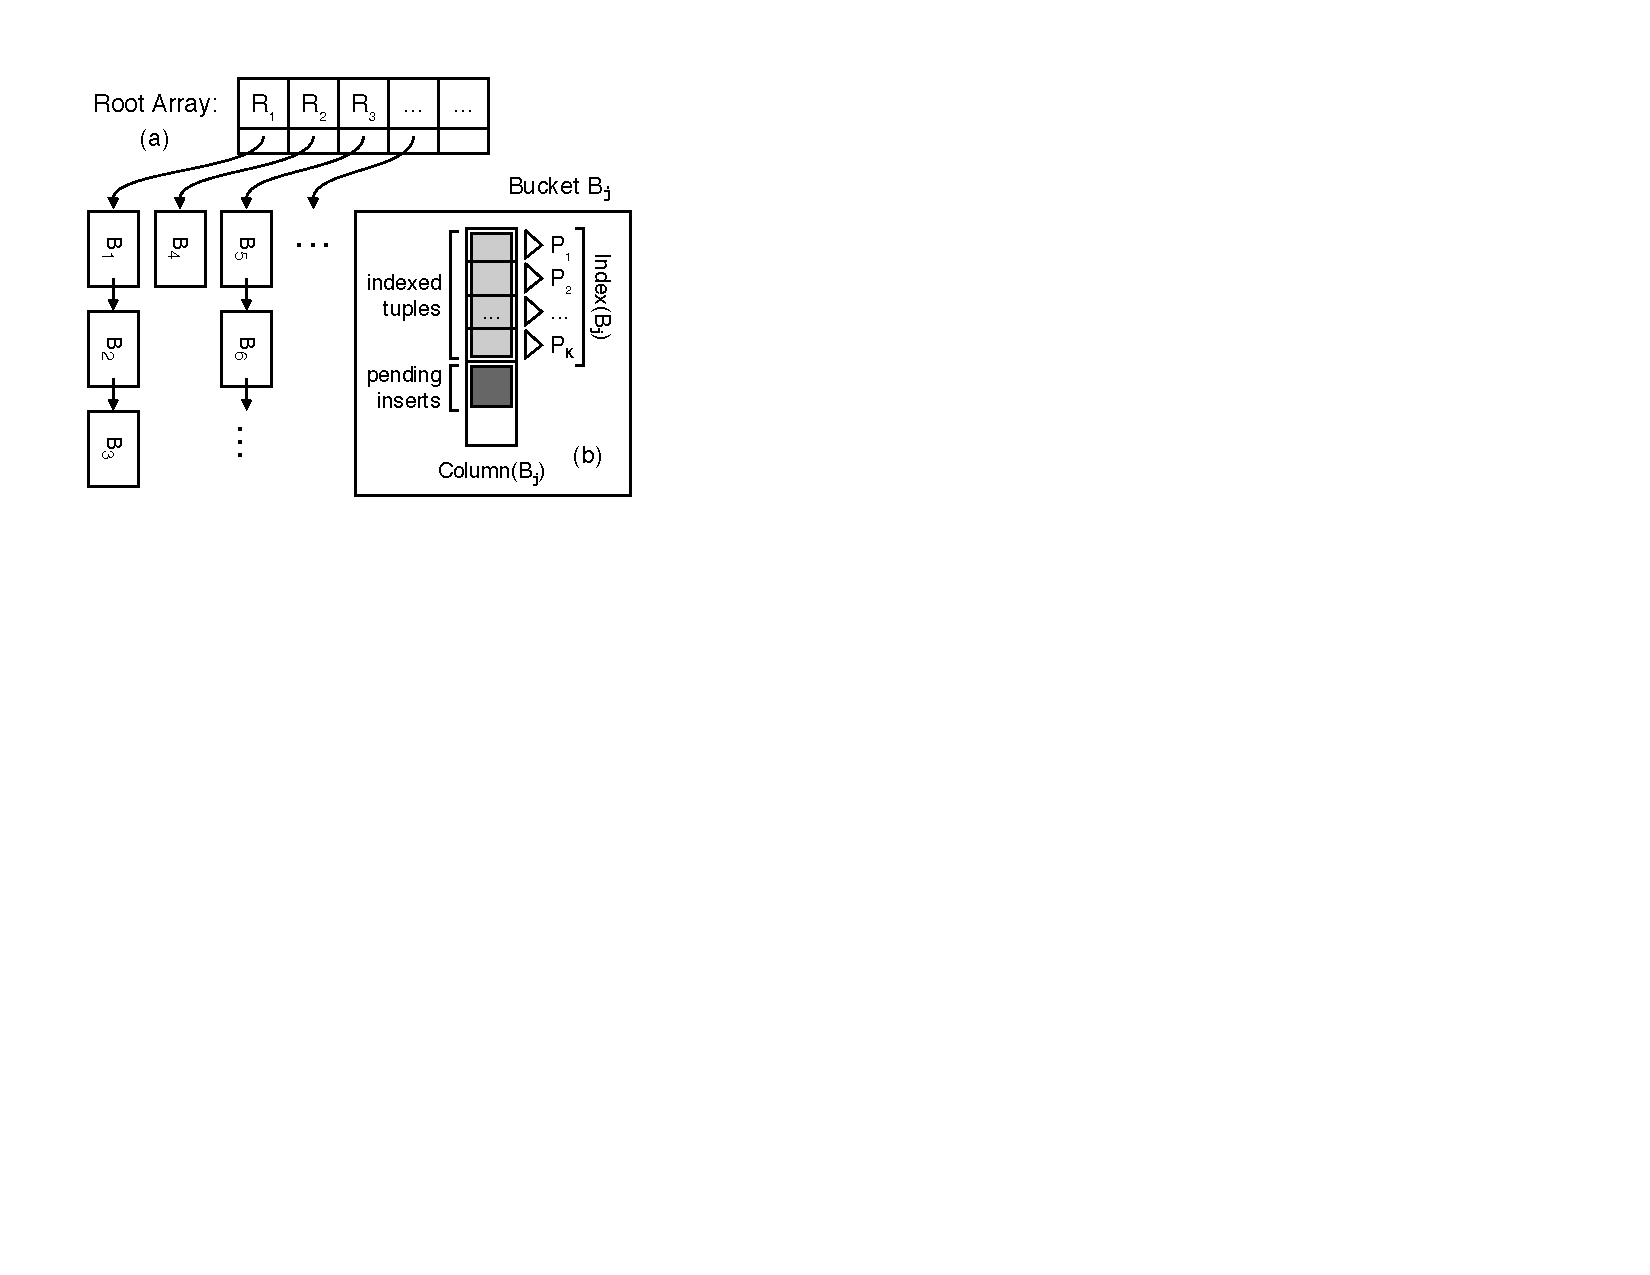
\includegraphics[width=1\columnwidth]{graphs/fig_crake.pdf}
\vspace{-1em}
\caption{The Comb structure.}
\vspace{-1em}
\label{F:crake}
}
\hfill
\hspace{-11.5em}%
\Fig[b]{.6\columnwidth}{%
\hspace{-.5em}%
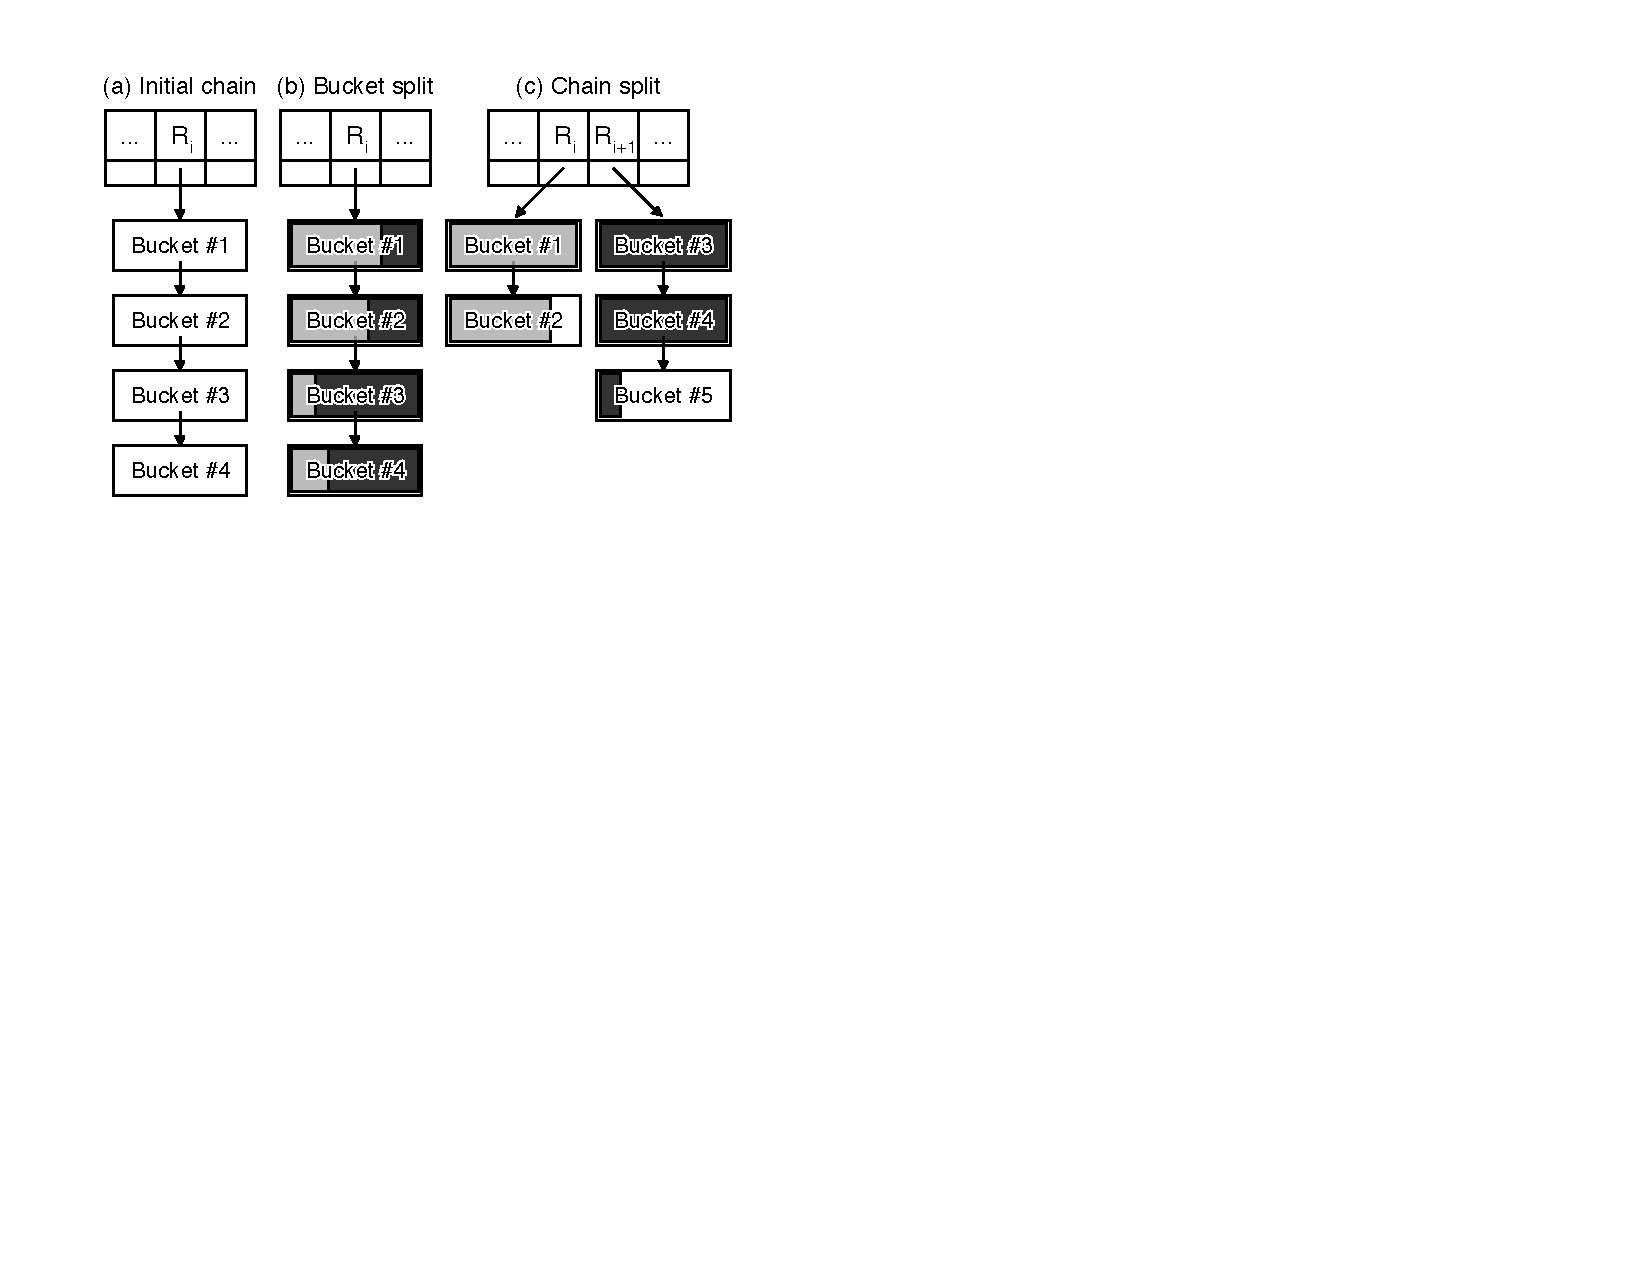
\includegraphics[width=1.05\columnwidth]{graphs/fig_crake_lazy.pdf}
\vspace{-1em}
\caption{Bucket chains and splits.}
\vspace{-1em}
\label{F:lazycrake}
}
\hfill
\hspace{-6.5em}%
\Fig[b]{.5\columnwidth}{%
\hspace{-6em}%
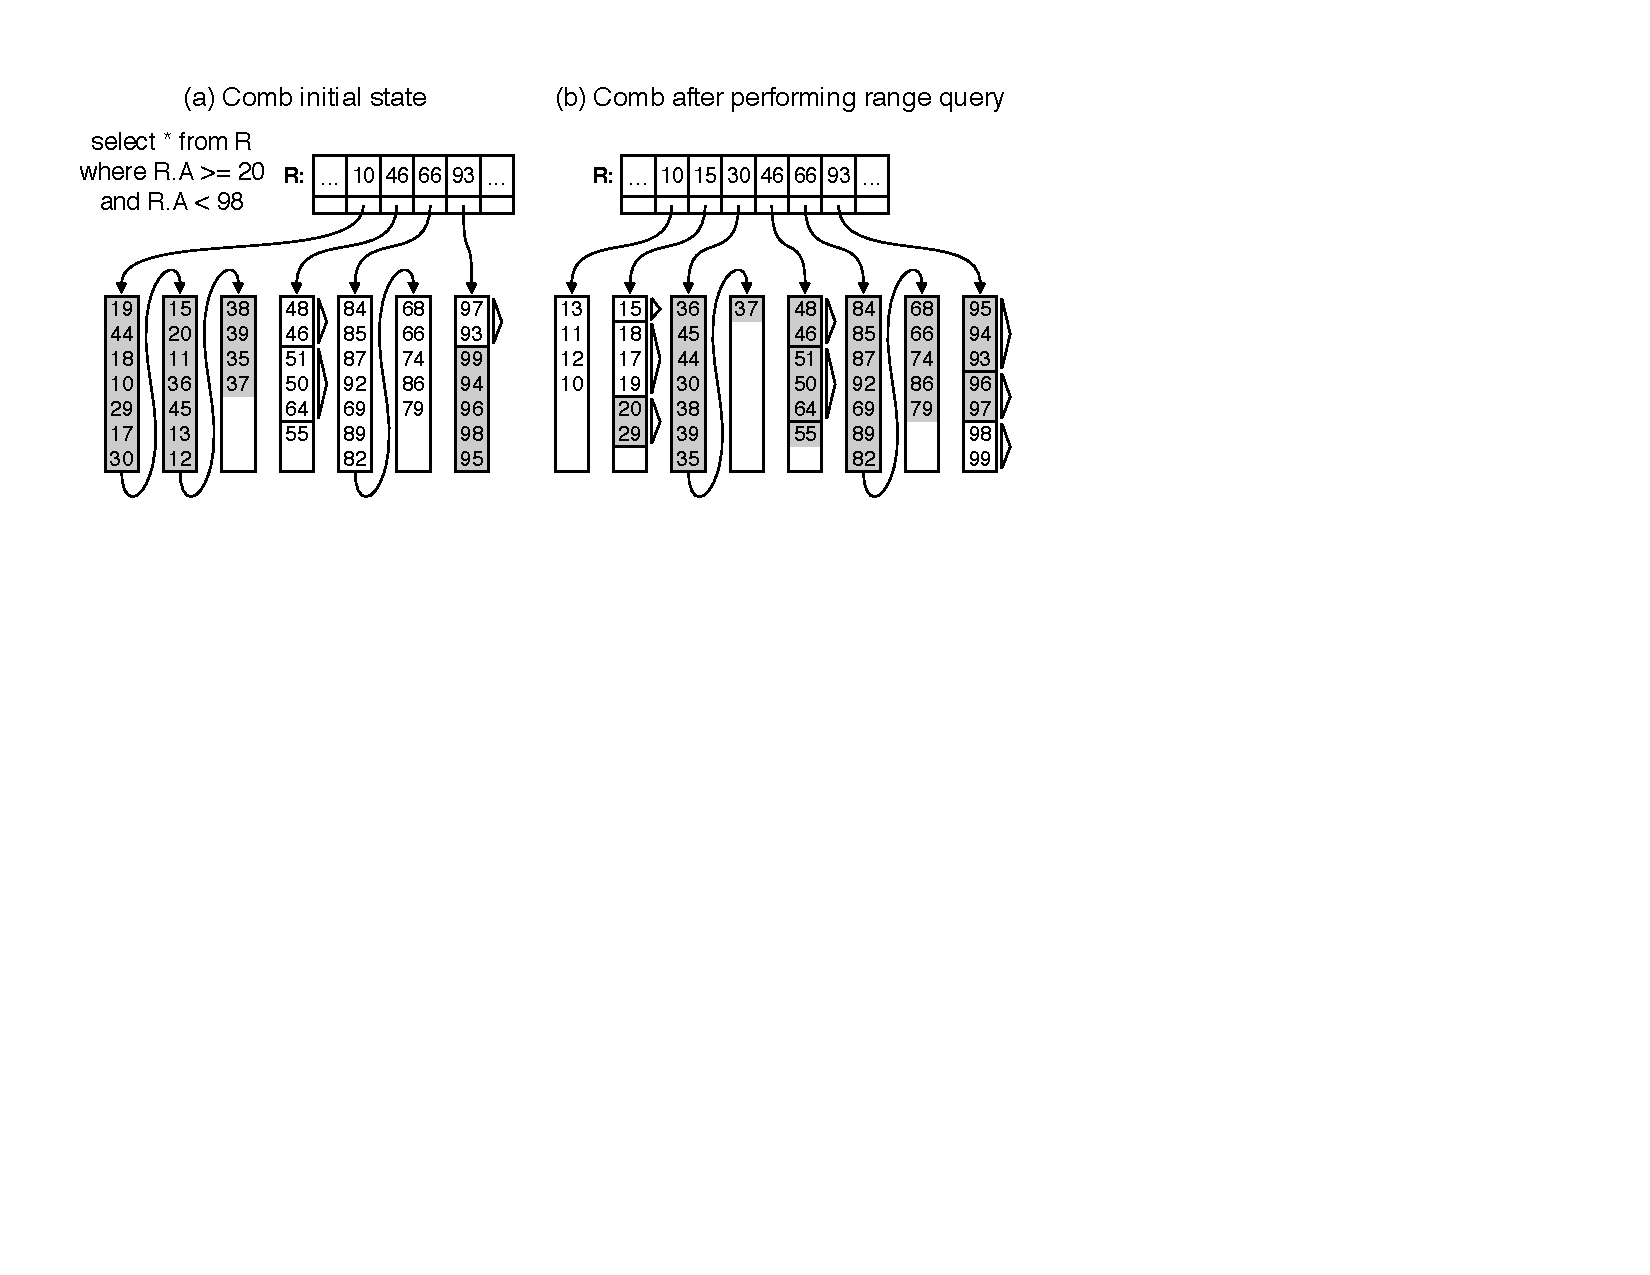
\includegraphics[width=1.8\columnwidth]{graphs/range_query.pdf}
\vspace{-1em}
\caption{Query example.}
\vspace{-1em}
\label{F:rangequery}
}
\end{figure*}

\subsection{Optimizing Existing Adaptive Indexing}
\label{sec:simple}

One way to deal with the non-resilience  problem of adaptive indexing is to patch existing 
adaptive indexing techniques so that they are less prone to performance degradation in long 
query sequences. One intuition is to restrict the growth of the index. 
By allowing the index to grow up to a certain size, and thus the column to be cracked up to a maximum number of pieces,
then there is a maximum traversal cost
as there is a maximum index depth for the tree part of the cracking index.
In addition, there is a maximum number of movements we have to do in order to 
update a cracking piece, as there is a maximum number of pieces (there are fewer pieces and thus bigger in size).
Below we introduce four directions on how to restrict the index size. 

\textbf{Crack-NoIndex.} This first approach allows cracking to continue working as normal with the exception 
that if a piece in the index  has reached a minimum size of $P_{min}$ tuples, then future queries continue to crack this
piece but do not inject this information in the tree part of the index.
The current query is answered as normal  but its refinements are not marked in the index and thus
cannot be exploited by future queries nor create excessive administration overheads.  

\textbf{Crack-Scan.} The next variation of cracking does not crack any more pieces 
in the column which reach  the threshold of $P_{min}$ tuples.
Instead, it scans a piece that it would normally crack.
As discussed in Section \ref{sec:problem}, a cracking range-select operator 
needs to touch at most two pieces at the edges of its target range. 
Thus, these extra scan actions add only a limited cost.
Contrary to the Crack-NoIndex approach,
Crack-Scan cannot return a view of the whole result and needs to materialize the qualifying values of the edge pieces.

\textbf{Crack-Sort.} The third alternative aims towards maximum read performance. 
When the piece size limit is reached, then a future query sorts completely a piece which should have been normally cracked.
The information that this piece is sorted is maintained in the tree index (an extra bit)
and future queries may simply binary search when their boundaries fall within this piece.

\textbf{Crack-Forget.} Finally, another interesting direction is to continue cracking as normal
with the addition that we ``forget" part of the indexing information in an adaptive way.
We can drop some of the partitioning knowledge only when necessary; this results in less pieces and thus less 
administrative overhead and update costs. In particular, in the spirit of adaptive indexing, 
we can drop pieces which are about to be updated and thus create extra costs.
This action is performed directly in the select operator during processing of a query that needs those pieces
and only if we exceed a maximum number of pieces in the index. With this strategy the index continuously adapts 
via cracking and still is able to avoid expensive updates in very well refined areas of the index.


\subsection{Comb: Cracking Over Malleable Buckets}
Optimizations and fine-grain variants of existing adaptive indexing techniques are limited
by fundamental choices in the original approaches. 
In Section \ref{sec:experiments}, we show that even though our optimized adaptive indexing designs
help with the resilience problem, the improvement is not enough.
% , still though there is potential to achieve significantly better performance.

\textbf{Comb.}
In this section, we introduce Comb (Cracking Over Malleable Buckets),
a novel adaptive indexing technique designed and tailored
to deal with the non-resilience problem of adaptive indexing when it comes to long strings of read and write queries,
while still maintaining all the good properties of previous adaptive indexing approaches.



A high level view of the Comb structure is shown in Figure \ref{F:crake}.
There are two fundamental components; (a) the root array and (b) the buckets.
A single Comb structure $Comb(C)$ maintains the contents of a single column $C$ in a column-store. 

\textbf{Root Array.}
The buckets in a Comb structure contain the actual tuples, while the root array serves the role
of guiding queries to the proper bucket.
As Figure \ref{F:crake} shows, each entry $R_i$ in the root array corresponds to a collection 
of one or more chained buckets $CB_i$.
Each root entry contains two variables. The first one is a physical pointer $Pointer(R_i)$
to the first bucket $B_i$ in chain $CB_i$.
The second one is the key $Key(R_i)$, which defines the starting point of the value range corresponding to bucket 
collection $CB_i$.
The root array is maintained sorted on its key values.

\textbf{Buckets.}
Each bucket in an index $Comb(C)$ is responsible for holding part of the tuples of the base column $C$.
Each chain of buckets $CB_i$, corresponding to root element $R_i$, holds all values in the range $[Key(R_i)$,$Key(R_{i+1}))$.
The value $Key(R_i)$ is the smallest value which is currently stored inside the buckets of $CB_i$.
The bottom part of Figure \ref{F:crake} shows how chains of malleable buckets 
connect to the root array and an instance of the internals of a bucket.

Inside each bucket $B_j$, there is a column, $Column(B_j)$, which holds the local tuples. 
This column is continuously cracked and reorganized as more queries arrive.
The last part of $Column(B_j)$ contains values which have been inserted but not yet merged with
the rest of the partitioned values in $Column(B_j)$.  

In addition, there is another array, $Index(B_j)$, which maintains the partitioning information for $Column(B_j)$;
it contains the pivots used for cracking on $Column(B_j)$ and the corresponding physical position
where each piece starts in $Column(B_j)$; it is equivalent to the root array with the difference that it is used 
for guiding through the local column. 
Array $Index(B_j)$ is maintained sorted.

Furthermore, there is a bit vector, $Sorted(B_j)$, which is aligned to $Index(B_j)$ and 
maintains information regarding whether a piece in $Column(B_j)$ is sorted or not (as in Crack-Sort). 

\textbf{Slicing.}
Comb carefully slices the data and the indexing information across buckets
and across the pieces in the local columns within each bucket.
The main target is to minimize the administrative costs as well as the access and update costs.

In a column of $N$ total tuples, each bucket may contain up to a maximum of $M$ tuples. 
In our experimental evaluation we found that performance is best when $M$ is such that each bucket fits in L1 cache.
Inside each bucket, each local column may be partitioned up to a maximum number of pieces $P$. 
By default, this is purposely kept small in the order of $P=128$ pieces per bucket to guarantee low update costs.
We will discuss the effect of those parameters later on.
In this way, the root array may contain up to $N/M$ entries, 
while each cracking piece in the local column inside each bucket contains on average  $M/P$ tuples. 

As we focus on main-memory environments, we design
Comb to have one root array for the following reason.
For example, consider a typical 2MB L2 cache; if the root array fits in L2,
our Comb implementation can index  
a raw column of 256GB integer values (including auxiliary row IDs).\footnote{
\small
When $N$ is even smaller,  a good choice is that of $M = sqrt(N)$,
balancing the size of the root array and buckets.
}
This is already more than conventional memory capacity and 
also more than the typical size of a single column in a database.
% Comb can already hold up to 
% If the root array fits in a typical 2MB L2-cache and we pick $M = sqrt(N)$, where $N$ is the size of indexed column $C$,
% then  Comb can hold up to $(2 MB)^2 ~= 512 GB$, 
% which is more than the conventional memory capacity and 
% also it is more than the typical size of a single column in a database.
Multi-level root arrays are certainly a possible extension.
However, this is beyond the scope of this paper.
% When $N$ is not so large as the above,
% a good choice of $M = sqrt(N)$ balancing the size of the root array
% and buckets.

\textbf{Insertions.}
Let us now discuss how new values are inserted in Comb.
Assume a new value $v$. 
Comb first searches its root array to find the bucket chain which contains $v$.
Since the root array is always sorted, searching is done via binary search and costs $O(\log(N/M))$.
The result bucket chain $CB_i$ is the one where $Key(CB_i)<=v<Key(CB_{i+1})$.
There are two cases when inserting a new value $v$. 

\textbf{Appending Inserts and Chaining Buckets.}
The first case is that the corresponding bucket chain $CB_i$ where $v$ belongs has enough space to accommodate $v$.
This means that the last bucket $B_j$ in $CB_i$ has at least one empty position.
In this case, the new value $v$ is simply appended at the pending inserts part of $Column(B_j)$.
This means that $v$ is placed immediately after the last indexed value of $Column(B_j)$ or immediately after the
last pending insert in the case that there are already pending inserts in $Column(B_j)$.
Holding both indexed values and pending inserts in $Column(B_j)$ means that a query which needs all values
in the value range stored in $B_j$ can blindly retrieve $Column(B_j)$. Analysis and merging is needed
only if a query needs to search within the range of $Column(B_j)$. 

The second case when inserting a value $v$ in a chain $CB_i$
is when the last bucket $B_j$ is full and no more values can be stored in $CB_i$.
In this case, Comb creates a new empty bucket $B_{new}$
and \emph{chains} $B_{new}$ to $B_j$. The new value is appended as a pending insert in $B_{new}$.
Examples of several buckets chained together are shown in Figures \ref{F:crake}, \ref{F:lazycrake} and \ref{F:rangequery}. 
All buckets under the same root entry $R_i$ contain values in $[Key(R_i),Key(R_{i+1}))$.

The design option to chain buckets under the same root entry guarantees low-cost insertions.
However, at the same time, the whole Comb structure should remain well adjusted to the workload to 
accommodate fast read access.
This means that there should be no individual long bucket chains in hot ranges.
Therefore, as we discuss later on, the buckets are {\em malleable}: 
queries can adaptively and on demand split chained buckets to balance
and optimize the value ranges which are relevant for the workload. 
An alternative design would be to eagerly split buckets during insertions.
However, we show in Section \ref{sec:experiments} that this is not a favorable design as it 
hurts the adaptive behavior of Comb. 



\textbf{Merging Inserts Inside a Bucket.}
Locally within each bucket $B_j$, insertions remain as pending insertions, stored at the last part of $Column(B_j)$
as shown in Figure \ref{F:crake}.
Insertions are merged with the indexed part of $Column(B_j)$ 
only when a query needs to refine the indexing information in $B_j$ or when deletes arrive in $B_j$. 
Comb merges local insertions in its cracked bucket columns using the cracking update algorithms 
as described in Section \ref{sec:problem} and in \cite{IKM:SIGMOD07}.
However, with Comb, the size of the columns as well as the partitioning depth of cracking in its local bucket 
columns are all kept under certain limits. This enables Comb to significantly restrict the update costs
by doing only small local actions within a single bucket when merging an update.
In addition, during query processing only the boundary pieces need to be updated;
we elaborate more on this important detail later in this section when we discuss about range queries.


\textbf{Initialization.}
Initializing a Comb index for an existing base column follows the procedure described for inserts above.
Starting with a single bucket, it continuously inserts new values and chains new buckets as they become full.
After loading a full column, and before any query has arrived,
the result is a multi-bucket structure as in Figure \ref{F:lazycrake}(a) with a single chain of buckets. 

\begin{figure}[t]
\begin{minipage}{4in}
{\small
\begin{tabbing}
16 16\= 16 \= 16 \= 16 \= 16 \= 16 \= 16 \= 16 \= 16 \= \kill
{\bf Algorithm} $\mathsf{RangeQuery}($low bound $v_1$, high bound $v_2)$\\
1.\>$lo$ = point\_query($v_1$)\\
2.\>$hi$ = point\_query($v_2$)\\
3.\>{\bf return} create\_view($lo$, $hi$) {\it// position of $v$ in Comb} \\
\\
{\bf function} $\mathsf{point\_query}($boundary value $v)$\\
4.\>{\bf if} (isEmpty($R$)) {\bf return} \{$|R|$, 0, 0\} {\it// past-the-end position}\\
5.\>$i$ = lower\_bound($R$, $v$) {\it// the first $i$ such that $Key(R_i) \geq v$}\\
6.\>$i$ = make\_standalone($i$, $v$)\\
7.\>$j$ = $Pointer(R_i)$\\
8.\>$k$ = crack($j$, $v$)\\
9.\>{\bf return} \{$i$, $j$, $k$\}\\
\\
{\bf function} $\mathsf{make\_standalone}($root index $i$, boundary value $v)$\\
10.\>{\bf while} (true) {\bf do}\\
11.\>\>$j$ = the first bucket pointed by $Pointer(R_i)$\\
12.\>\>{\bf if} ($B_j$ does not have a next bucket) {\bf break}\\
13.\>\>stochastic\_split\_chain($i$)\\
14.\>\>{\bf if} ($v \geq Key(R_{i+1}$)) $i = i+1$ {\it// adjust root index to where $v$ is}\\
15.\>{\bf return} $i$\\
\\
{\bf function} $\mathsf{stochastic\_split\_chain}($root index $i)$\\
16.\>$pv$ = pick\_random\_pivot(i) {\it// stochastic crack pivot value}\\
17.\>{\bf for} ($j$ = $|R|-1$; $j>i$; $j$-{}-) {\bf do} {\it// shift elements at $j > i$ to the right}\\
18.\>\>$Pointer(R_{i+1}) = Pointer(R_i)$\\
19.\>\>$Key(R_{i+1}) = Key(R_i)$\\
20.\>$|R|$ = $|R|+1$ {\it// increase the number of stored tuples |R|}\\
21.\>$Key(R_{i+1})$ = $pv$ {\it// set the smallest value in $R_{i+1}$ bucket chain}\\
22.\>perform split\_chain($i$, $pv$) which split a bucket chain pointed by\\
\>$Pointer(R_i)$, transferring tuples with values $\geq pv$ to buckets\\
\>in chain $R_{i+1}$ (implementation details are in Section \ref{sec:splitting})\\
\\
{\bf function} $\mathsf{crack}($bucket number $j$, boundary value $v)$\\
23.\>flush\_pending\_inserts($j$)\\
24.\>let $P_v$ = the (local) cracker piece of $B_j$ where $v$ is in\\
25.\>{\bf while} ($|P_v|$ > $CRACK\_AT$) stochastic\_split($P_v$) {\it// perform DD1R}\\
26.\>{\bf if} ($P_v$'s sorted flag is not set)\\
27.\>\>{\bf if} (this is a read query) sort the piece $P_v$ and set its sorted flag\\
28.\>\>{\bf else} {\bf return} the position of $v$ in $P_v$ via linear scan\\
29.\>{\bf return} the position of $v$ in $P_v$ via binary search\\
\\
{\bf function} $\mathsf{flush\_pending\_inserts}($bucket number $j)$\\
30.\>if (no local cracker index) consider all tuples are merged and {\bf return}\\
31.\>do merge insert completely to all the (local) pending tuples in $B_j$\\
32.\>unset the sorted flags of the pieces that are touched during merging\\
\end{tabbing}
}
\end{minipage}
\vspace{-1em}
\caption{Range query in Comb.}\label{algo:pointquery}
\vspace{-1.5em}
\end{figure}

% We define an iterator as a tuple with 3 values: \{$i$, $j$, $k$\}.
% An iterator is used to locate the position of a tuple.
% $i$ is the index of the root array, $j$ is the bucket number,
% and $k$ is the position of the tuple in the bucket $B_j$.

% $RangeQuery(v_1,v_2)$ returns a view consisting of an iterator such that positions before 
% the iterator is $<v$ and positions after the iterator is $\geq v$.
% The iterator is constructed by first finding the index of the root array ($i$)
% containing the tuple with value $v$ (line 2).
% The bucket pointed by the root array must be standalone (line 3)
% otherwise the bucket chain is split until it is standalone (line 8-11). 
% Next we retrieve the (standalone) bucket number ($j$) pointed by the root array (line 4).
% The bucket's array is then cracked on value $v$ and the cracked position is at $k$.
% We now have all the necessary ingredients to construct the pointer \{$i$, $j$, $k$\}.


\textbf{Deletes.}
For robustness reasons deletes follow an eager strategy and are applied 
in one go in each bucket. If we want to delete a value $v$, we first locate the
corresponding bucket $B_i$. Then, first all pending, if any, local inserts are merged
and subsequently we locate and delete $v$ by shuffling the tuple at the end of its
piece as described in Section \ref{sec:problem}.
In case there are several chained buckets under the same root entry,
then all chained buckets are updated.

An alternative strategy would be to allow deletes to remain pending and only merge them later on
as we do with inserts. However, as we show later on in Section \ref{sec:experiments}, 
this is not a robust solution as it can severely hurt read queries. 

\textbf{Continuous Adaptation.}
Comb is an adaptive index. As such queries are the driving force which shapes the index.
As more queries arrive, the index is continuously refined to adjust to the workload patterns.
The more a value range is queried, the more resolution the index adopts in this range.
At the same time, value ranges not queried are seen in a much more coarse resolution until relevant queries arrive.

\textbf{Adaptation During Queries.}
We now proceed to describe how select operations work  on top of Comb.
Figures \ref{F:lazycrake} and \ref{F:rangequery}  show how Comb is adaptively refined after a read query.
Figure \ref{F:lazycrake} shows how a single chain is split into two new ones,
while Figure \ref{F:rangequery} shows the end result of a full range query after all its split and cracking actions.
The chains at the borders of the requested range are adaptively split, while the buckets
at the very borders are cracked using the query bounds. 
This way, Comb adapts both at a global level by splitting chains at hot workload areas
and at a local level by refining the index information within buckets in hot areas.
The work performed is minimized as only the 2 boundary chain buckets need to be touched, i.e., the chains where the query bounds fall;
all chains and buckets in between are known to qualify so there is no need to be refined 
(this is similar to the discussion we did for cracking 
in Figure \ref{F:CrackExample} and Section \ref{sec:problem}).
Given that we do not have to refine all chains in between the query boundaries, 
this also means that we do not have to merge local updates in their respective buckets 
as we need all qualifying values anyway (both indexed and non-indexed values).
This is why a more lazy approach to inserts is beneficial.
With deletes, however, we need to guarantee there are no deletes leftover across all qualifying buckets
both in the borders of the queried range and in between. Being lazy creates excessive costs at query time, hence,
we choose eager deletes locally within each bucket.
We revisit the last two points in Section \ref{sec:experiments}. 


\textbf{Querying Comb.}
The algorithm for a Comb range select is described in detail Algorithm \ref{algo:pointquery}.
%In our pseudocode presentation, array indexing is also denoted by subscripts, e.g.
%$R[i]$ by $R_i$ (line 7),
%and $|x|$ is the size of array $x$, so $|R| = |R| + 1$ increases the array $R$ by 1.
Assume a select operator requesting all values in $[low,high]$ from column $C$.
Comb first searches its root array to find the bucket chain $CB_{low}$ 
which contains $low$ and the chain $CB_{high}$ which contains $high$.
Since the root array is always sorted, searching is done via binary search and costs $O(\log(N/M)$.

For ease of presentation, assume first that both boundary chains contain one bucket each. 
For chain $CB_{low}$, the select operator searches within the single bucket $B_{low}$ for $low$.
In this way, for the single bucket $B_{low}$ in $CB_{low}$,
it does a lookup in $Index(B_{low})$ to find the piece in $Column(B_{low})$ where $low$ is contained.
Given that $Index(B_{low})$ is sorted, the search is done via a binary search action 
(similar to searching the root array). This costs $O(\log(P))$.
Once we know the corresponding piece $P_{low}$, then the next action depends on whether 
the size of the piece has reached the minimum allowed size ($M/P$) (denoted as $CRACK\_AT$ in Algorithm \ref{algo:pointquery}).
In the case that we have already reached the piece size limit, then we check (in $Sort(B_{low})$) whether
$P_{low}$ is already sorted. If yes, then we simply binary search in $P_{low}$ to find $low$.
Otherwise, we first sort $P_{low}$ in-place and then binary search for $low$. 
The respective piece is marked in bit vector  $Sort(B_{low})$. 
If the size of the piece is still above the size threshold, 
then $P_{low}$ is recursively cracked using random pivots until it reaches a small enough size
where it can be sorted with a small cost.
For this step, Comb uses the stochastic cracking algorithm (DDR) which is shown to be robust \cite{StochasticCracking}.
$Index(B_{low})$ is updated with a new entry for the new pieces created.
The most expensive case is when this is the very first query in $B_{low}$ and $B_{low}$ is full. 
Then, we need to reorganize $Column(B_{low})$ touching all $M$ tuples.

The above procedure is repeated by analogy for $CB_{high}$ and $high$.
Once we have reorganized the boundary chains, then all chains and buckets in between form the result
as shown in the example of Figure \ref{F:rangequery} (qualifying tuples are marked with grey color).
The total cost of a query is $O(\log(N/M) + \log(P) + M)$.


\textbf{Adaptive Splits During Queries.}
In the case that a boundary chain where a query bound $b$ falls in contains more than one buckets, then 
a query adaptively and recursively splits this chain until the boundary chain where $b$ falls in 
remains with a single bucket.  
In order to split a chain $CB_i$ as the one in Figure \ref{F:lazycrake}(a), 
the first step is to choose a random pivot $rv$. 
The pivot $rv$ is used to crack, i.e., to physically reorganize all chained
buckets in $CB_i$, such as to split the values in two partitions per chained bucket; 
one partition contains all values $x<rv$ and the second partition contains all values $x>=rv$.
The result of this step is shown in Figure \ref{F:lazycrake}(b).
Now we can create two new sets of chained buckets as shown in Figure \ref{F:lazycrake}(c) where the right set
of buckets is under a new root entry on the random pivot which was chosen for the split.
Bound $b$ falls in one of those chained buckets. The process of adaptive splitting continues recursively
until the chain where $b$ falls in is a single bucket and thus no more splits are required.

We could split directly on $b$ as a pivot, 
but then Comb would be vulnerable to unfavorable workload patterns, as it has been shown for adaptive indexing in \cite{StochasticCracking}. 
Thus, we opt to choose random pivots and keep splitting until there is only one bucket in the 
chain that contains $b$ so as to achieve robustness. 
The extra splitting overhead we pay affords more robust performance in subsequent queries.

\begin{figure}[t]
\begin{minipage}{4in}
{\small
\begin{tabbing}
16 16\= 16 \= 16 \= 16 \= 16 \= 16 \= 16 \= 16 \= 16 \= \kill
{\bf Algorithm} $\mathsf{Crack::split\_chain}($root index $i$, pivot value $v)$\\
1.\>$A$ = new array of pair$\langle $partition\_position, bucket\_index$\rangle$\\
2.\>{\bf foreach} bucket $B_j$ chained by $Pointer(R_i)$ {\bf do}\\
3.\>\>$pos$ = std::partition($Column(B_j)$, $v$)\\
4.\>\>$A$.push($\langle pos$, $j\rangle$) {\it // appends to the end of the array}\\
5.\>sort\_descending($A$) {\it // to minimize data exchanges below}\\
6.\>$left\_chain$ = new bucket chain\\
7.\>$right\_chain$ = new bucket chain\\
8.\>$k$ = 0, $n$ = $|A|-1$\\
9.\>{\bf while} ($k < n$) {\bf do}\\
10.\>\>let $\langle r,p\rangle$ denote $A_k$\\
11.\>\>let $\langle s,q\rangle$ denote $A_n$\\
12.\>\>$a$ = $Column(B_p)$, $b$ = $Column(B_q)$\\
13.\>\>$m$ = min($|B_p| - r$, $s$)\\
14.\>\>{\bf while} ($m>0$) {\bf swap}($a_r$, $b_s$), $r$ = $r+1$, $s$ = $s-1$, $m$ = $m-1$\\
15.\>\>{\bf if} ($r$ == $|B_p|$) $left\_chain$.append\_bucket($B_{p}$), $k$ = $k+1$\\
16.\>\>{\bf if} ($s$ == 0) $right\_chain$.append\_bucket($B_{q}$), $n$ = $n-1$\\
17.\>let $\langle r,p\rangle$ denote $A_k$\\
18.\> $a$ = $Column(B_p)$\\
19.\>{\bf if} ($r$ == $|B_p|$) $left\_chain$.append\_bucket($B_{p}$)\\
20.\>{\bf else if} ($r$ == $0$) $right\_chain$.append\_bucket($B_{p}$)\\
21.\>{\bf else}\\
22.\>\>$q$ = create a new empty bucket\\
23.\>\>move tuples at positions [$r$,$|B_p|$) in $Column(B_p)$ to $B_q$\\
24.\>\>$left\_chain$.append\_bucket($B_{p}$)\\
25.\>\>$right\_chain$.append\_bucket($B_{q}$)\\
26.\>$Pointer(R_i)$ = $left\_chain$\\
27.\>$Pointer(R_{i+1})$ = $right\_chain$\\
\\
{\bf function} $\mathsf{std::partition}($column $A$, pivot value $v)$ {\it // from C++ STL}\\
28.\>$first$ = $0$, $last$ = $|A|$\\
29.\>{\bf while} (true) {\bf do}\\
30.\>\>{\bf while} (true) {\bf do}\\
31.\>\>\>{\bf if} ($first$ == $last$) {\bf return} $first$\\
32.\>\>\>{\bf else if} ($A_{first}$ < $v$) $first$ = $first$+1\\
33.\>\>\>{\bf else break}\\
34.\>\>$last$ = $last$-1\\
35.\>\>{\bf while} (true) {\bf do}\\
36.\>\>\>{\bf if} ($first$ == $last$) {\bf return} $first$\\
37.\>\>\>{\bf else if} ($A_{last}$ $\ge$ $v$) $last$ = $last$-1\\
38.\>\>\>{\bf else break}\\
39.\>\>{\bf swap}($A_{first}$, $A_{last}$)\\
40.\>\>$first$ = $first$+1\\
\end{tabbing}
}
\end{minipage}
\vspace{-1em}
\caption{Splitting Comb buckets using cracking.}\label{algo:crack}
\vspace{-1.5em}
\end{figure}


% // the bucket has been partitioned based on the value P.
% // the cracker index position is at L

% line 3 destroys $B_j$ local cracker indexes


\begin{figure}[t]
\begin{minipage}{4in}
{\small
\begin{tabbing}
16 16\= 16 \= 16 \= 16 \= 16 \= 16 \= 16 \= 16 \= 16 \= \kill
{\bf Algorithm} $\mathsf{Fission::split\_chain}($root index $i$, pivot value $v)$\\
1.\>$chain[0]$ = new bucket chain\\
2.\>$chain[1]$ = new bucket chain\\
3.\>{\bf foreach} bucket $B_j$ in chain $Pointer(R_i)$ {\bf do}\\
4.\>\>{\bf while} ($B_j$ is not empty) {\bf do}\\
5.\>\>\>$t$ = $B_j$.pop\_back() {\it // returns and remove the last tuple}\\
6.\>\>\>$chain[t \ge v]$.append\_tuple($t$) {\it // chains new bucket if full}\\
7.\>$Pointer(R_i)$ = chain[0]\\
8.\>$Pointer(R_{i+1})$ = chain[1]
\end{tabbing}
}
\end{minipage}
\vspace{-1em}
\caption{The Fission algorithm.}\label{algo:fission}
\vspace{-1.5em}
\end{figure}

% Tuples that are < P are copied to the left bucket, the rest to the right bucket.


\begin{figure}[t]
\begin{minipage}{4in}
{\small
\begin{tabbing}
16 16\= 16 \= 16 \= 16 \= 16 \= 16 \= 16 \= 16 \= 16 \= \kill
{\bf Algorithm} $\mathsf{Fusion::split\_chain}($root index $i$, pivot value $v)$\\
1.\>$chain$ = $Pointer(R_i)$\\
2.\>$left\_chain$ = new bucket chain\\
3.\>$right\_chain$ = new bucket chain\\
4.\>$p$ = -1, $q$ = -1 {\it// are the left and right bucket number respectively}\\
5.\>$hi$ = new array {\it// list of indexes of tuples in $B_p$ that are $\ge$ $v$}\\
6.\>$lo$ = new array {\it// list of indexes of tuples in $B_q$ that are $< v$}\\
7.\>{\bf while} (true) {\bf do}\\
8.\>\>{\bf if} (both $hi$ and $lo$ are not empty) {\bf do} {\it// fuse $B_p$ and $B_q$ using $lo$ and $hi$}\\
9.\>\>\>$a$ = $Column(B_p)$, $b$ = $Column(B_q)$\\
10.\>\>\>{\bf for} ($m$ = min($|hi|$, $|lo|$); $m>0$; $m$-{}-) {\bf do}\\
11.\>\>\>\>$r$ = $hi$.pop\_back() {\it// index of the tuple in $B_p$ to be moved to $B_q$}\\
12.\>\>\>\>$s$ = $lo$.pop\_back() {\it// index of the tuple in $B_q$ to be moved to $B_p$}\\
13.\>\>\>\>swap($a_r$, $b_s$) {\it// swap tuples between the left and right bucket}\\
15.\>\>\>{\bf if} ($hi$ is empty) $left\_chain$.append\_bucket($B_p$), $p$ = -1\\
16.\>\>\>{\bf if} ($lo$ is empty) $right\_chain$.append\_bucket($B_q$), $q$ = -1\\
17.\>\>{\bf else if} ($p$ == -1)\\
18.\>\>\>{\bf if} ($chain$ is empty) {\bf break; else} $p$ = $chain$.pop\_front()\\
19.\>\>{\bf else if} ($hi$ is empty)\\
20.\>\>\>{\bf for} ($j=0$; $j<|B_p|$; $j$++) {\it// no branch prediction}\\
21.\>\>\>\>$hi_{|hi|}$ = $j$, $|hi|$ = $|hi| + (Column(B_p)_j \ge v)$\\
22.\>\>\>{\bf if} ($hi$ is empty) $left\_chain$.append\_bucket($B_p$), $p$ = -1\\
23.\>\>{\bf else if} ($q$ == -1)\\
24.\>\>\>{\bf if} ($chain$ is empty) {\bf break; else} $q$ = $chain$.pop\_front()\\
25.\>\>{\bf else if} ($lo$ is empty)\\
26.\>\>\>{\bf for} ($j=0$; $j<|B_q|$; $j$++) {\it// no branch prediction}\\
27.\>\>\>\>$lo_{|lo|}$ = $j$, $|lo| = |lo| + (Column(B_q)_j < v)$\\
28.\>\>\>{\bf if} ($lo$ is empty) $right\_chain$.append\_bucket($B_q$), $q$ = -1\\
29.\>{\bf if} ($q$ != -1) $p$ = $q$;\\
30.\>{\bf if} ($p$ != -1)\\
31.\>\>{\bf if} ($B_p$ is empty) free bucket $B_p$\\
32.\>\>{\bf else}\\
33.\>\>\>pos = std::partition($Column(B_p)$, $v$)\\
34.\>\>\>{\bf if} (pos == 0) $right\_chain$.append\_bucket($B_p$)\\
35.\>\>\>{\bf else if} (pos == $|B_p|$) $left\_chain$.append\_bucket($B_p$)\\
36.\>\>\>{\bf else}\\
37.\>\>\>\>$q$ = create new bucket\\
38.\>\>\>\>move tuples at positions [$pos$,$|B_p|$) in $Column(B_p)$ to $B_q$\\
39.\>\>\>\>$left\_chain$.append\_bucket($B_p$)\\
40.\>\>\>\>$right\_chain$.append\_bucket($B_q$)\\
41.\>$Pointer(R_i)$ = $left\_chain$\\
42.\>$Pointer(R_{i+1})$ = $right\_chain$
\end{tabbing}
}
\end{minipage}
\vspace{-1em}
\caption{Fusion algorithm.}\label{algo:fusion}
\vspace{-2.5em}
\end{figure}

%             // generate a list of indexes of tuples \\
%  // which value is >= P in the left bucket.\\
% / store the indexes in hi[] temporary array.\\
%  // there is no branch prediction here.\\
%  // this loop work better with -funroll-loops enabled.\\


%              // generate a list of indexes of tuples\\
%   // which value is < P in the right bucket.\\
% // store the indexes in lo[] temporary array.\\
%   // there is no branch prediction here.\\
%   // this loop work better with -funroll-loops enabled.\\


\newpage
\textbf{Example.}
Figure \ref{F:rangequery} shows an example of a range query in Comb.
It shows the initial state and the final state after the index adapts to the query.
The query asks for all values in $[20,98)$.
Initially, there are 4 bucket chains linked in the root array as shown in Figure \ref{F:rangequery}(a).
The first chain under $key=10$ contains 3 chained buckets. 
The second chain under $key=46$ contains a single bucket which is already cracked in two pieces (indicated by triangles)
and also contains 1 pending insert value $val=55$. 
The third chain contains 2 chained buckets, while the fourth one is again a stand-alone bucket.
In order to answer the range query, Comb first searches for low bound, $low=20$
in the initial state in Figure \ref{F:rangequery}(a). 
This lies in the first chain of buckets (between root entries with $key=10$ and
 $key=46$).
Comb adaptively splits this chain in a stochastic fashion
into 3 new chains as shown in Figure \ref{F:rangequery}(b) with keys 10, 15
and 30. The bound $low=20$ falls in [15,30) so it falls in the second chain in Figure \ref{F:rangequery}(b)
under $key=15$. Then, this chain is cracked using $val=20$ as pivot. 
The grey region in the buckets in  Figure \ref{F:rangequery}(a) shows which tuples
are touched from the initial state during the query process.
An important feature of Comb is that
the chain under $key=46$ from Figure \ref{F:rangequery}(a) is untouched --
it is not accessed, cracked and its pending inserts are not merged 
although it qualifies for the result.
To answer the query, it suffices
to fetch all values in the bucket regardless of the order or the partitioning information. 
The same holds for the chain under $key=66$ which remains as a chain of two unindexed chained buckets.
Finally, using the high bound of the query $high=98$, Comb adapts the chain under $key=93$ 
and cracks it using $val=98$ as pivot (the 98 is not inclusive).
The tuples which qualify for the query result are shown by the grey area
in  Figure \ref{F:rangequery}(b).
%The query result is marked by the grey area between the buckets that contain the low and high bounds
%and all the buckets in between.



\subsection{Bucket Splitting}
\label{sec:splitting}

The {\em malleability} of buckets, i.e., their capacity to be split and re-combined, 
is one of the most crucial properties in Comb.
Thanks to this malleability, we can maintain a well balanced structure which is easy to access and update.
The key action is that of partitioning a collection of chained buckets into roughly two equal pieces each, i.e., 
the step shown in Figure \ref{F:lazycrake}(b).

The partitioning of each bucket can be done using a standard partitioning algorithm
for partitioning columns (similar to what cracking is using). 
The resulting algorithm, $Crack::split\_chain$, which splits a chain of buckets is shown in Figure \ref{algo:crack}.
It first splits all buckets in a chain in two pieces based on the same (random) pivot and then creates two new chains 
to place the resulting pieces, trying to minimize data movement as much as possible.
%We show in our experimental analysis in Section \ref{sec:experiments} 
%that there are more opportunities to gain a significant advantage in performance
%than extending a standard partitioning algorithm.


\textbf{Fission.}
We discuss two new alternative designs which are optimized to split chains and buckets in Comb.
The first algorithm, called \emph{Fission}, is shown in 
Figure \ref{algo:fission}. Its main characteristic is that it splits buckets without using any branches;
this removes the hazard of branch mispredictions which, as we show later on, 
is excessive when splitting buckets in two half pieces.
Splitting buckets in half is preferable in order to minimize the number of splits required
(since adaptive splitting works recursively).

\textbf{Fusion.}
Still though there are more opportunities to improve this crucial Comb operation further.
We propose a new algorithm, called \emph{Fusion}, to split Comb chains.
The goal is to minimize both data movement and branch misprediction cases.
The main idea is that it works in two passes over the data which turns
out to be faster in modern architectures compared with a single pass.
The first pass marks which tuples need to be moved in a branch-free way, 
while the second pass implements these data movements in-place. 
The details are in Algorithm \ref{algo:fusion}.
Since the all to be moved tuples have been marked in the first pass, Fusion can minimize data movements
as in the second pass it knows exactly which tuples in each bucket need to be moved and where they should go.
 








%\begin{figure*}[t]
\Fig[b]{.8\columnwidth}{%
\hspace{-.6em}%
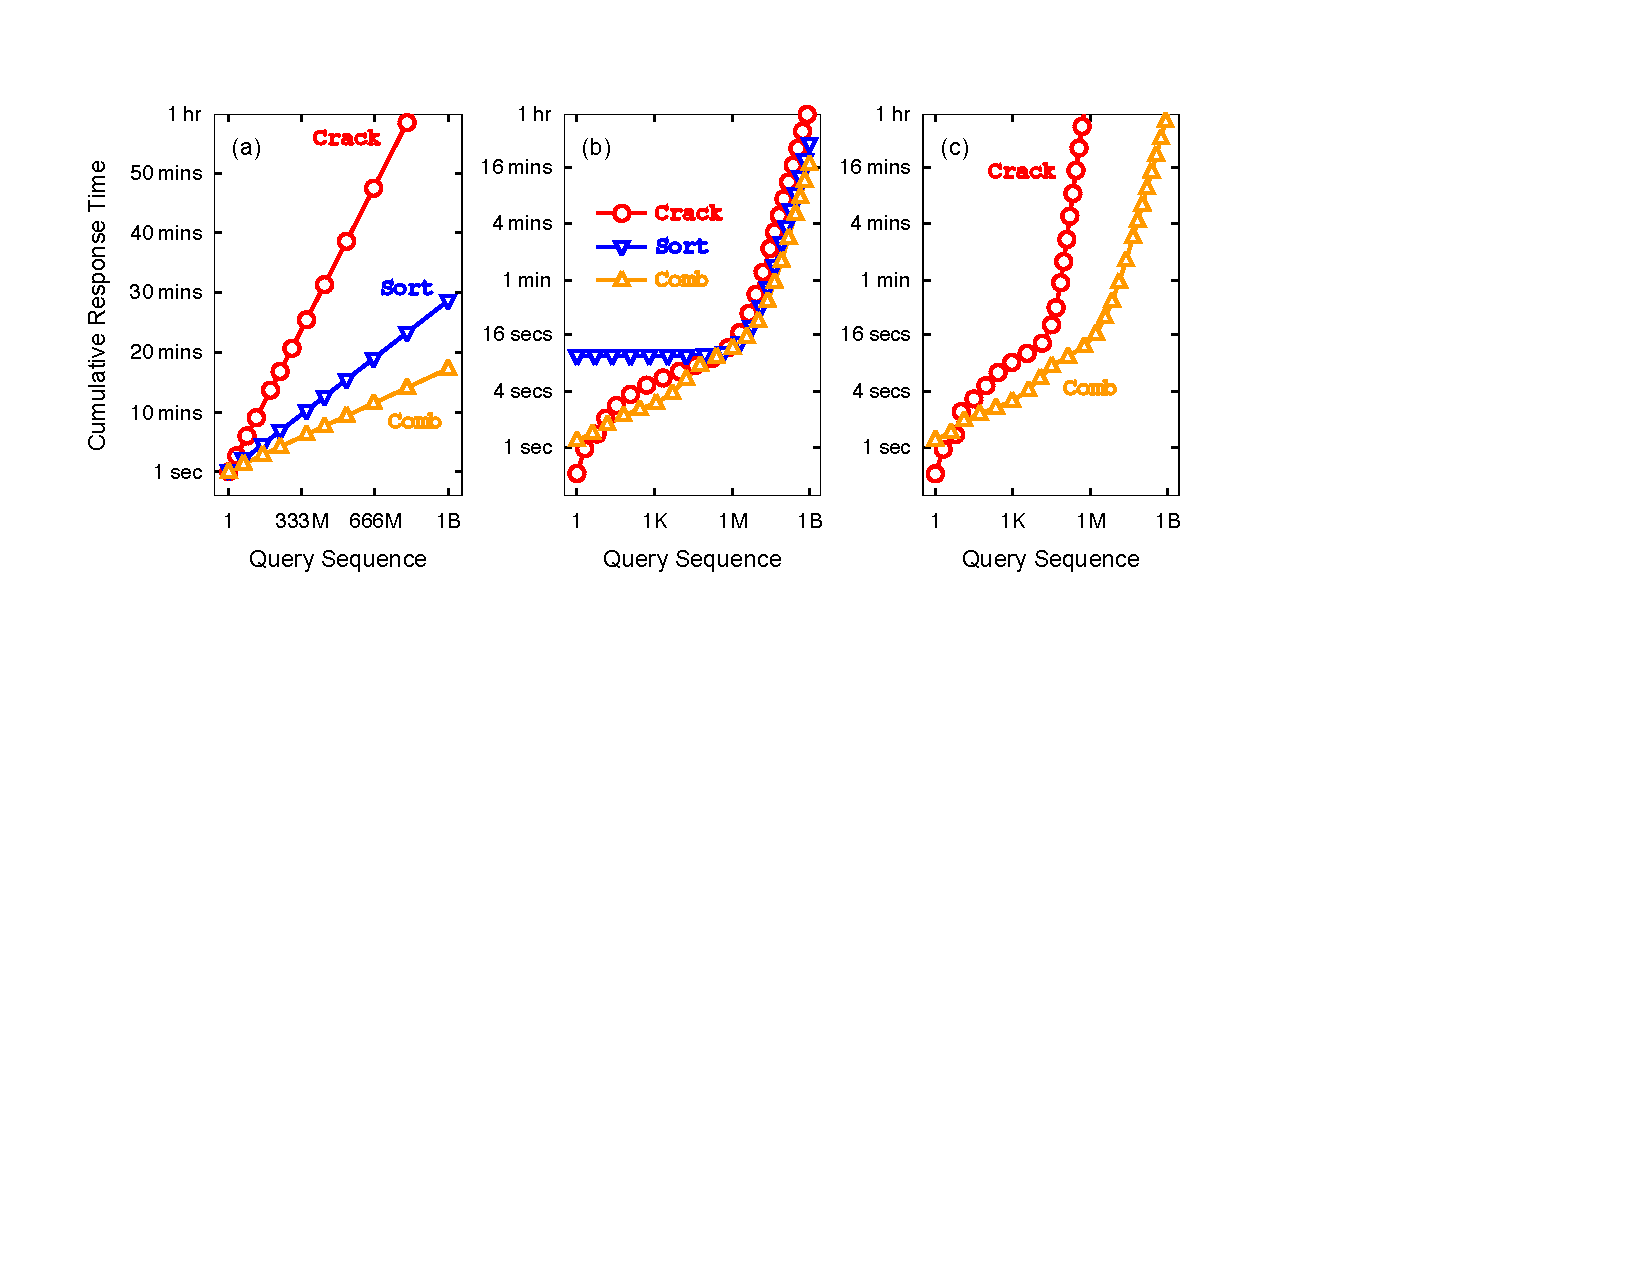
\includegraphics[width=1.35\columnwidth]{graphs/fig_basic_crake.pdf}%
\vspace{-1em}
\caption{Resilient adaptive indexing with Comb.}
\vspace{-1em}
\label{F:BasicPerQueryComb}
}
\hfill
\hspace{5.5em}%
\Fig[b]{.55\columnwidth}{%
\hspace{2em}%
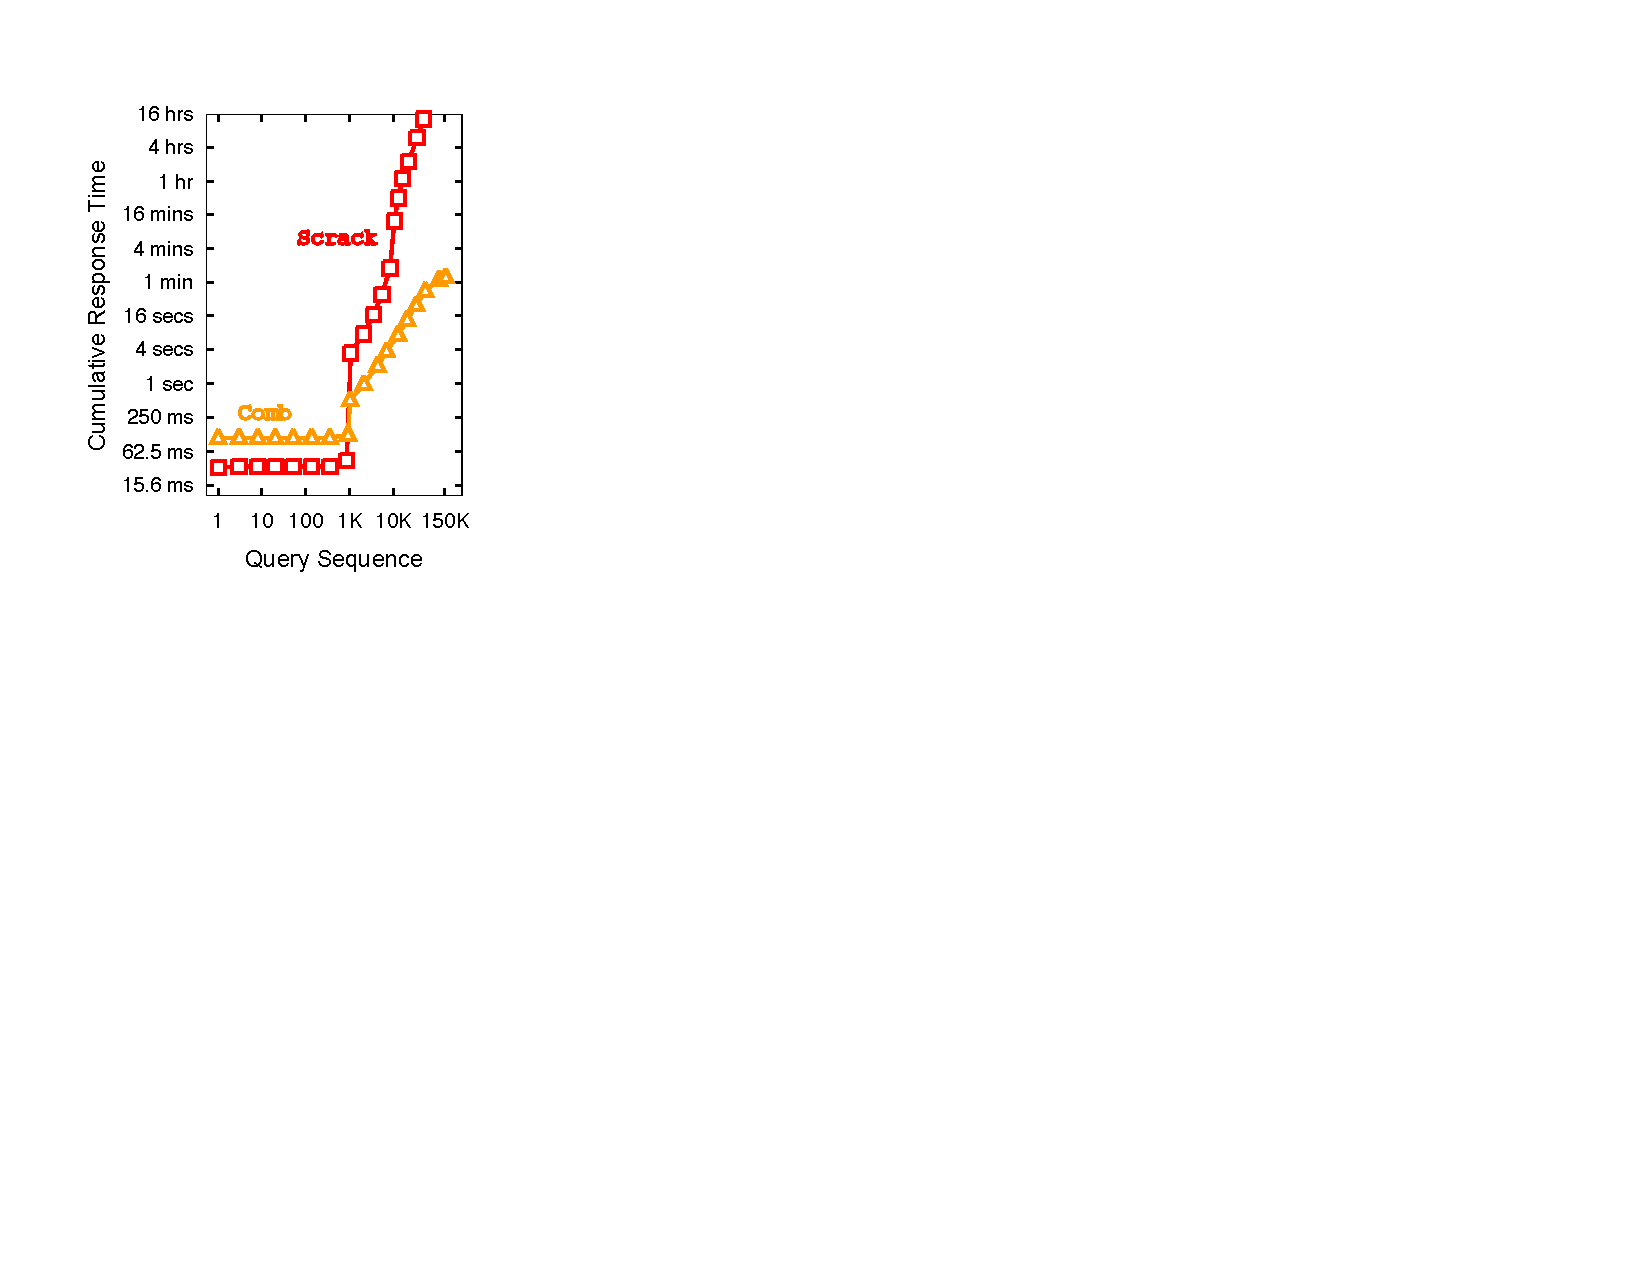
\includegraphics[width=.7\columnwidth]{graphs/fig_skyserver.pdf}%
\vspace{-1em}
\caption{SkyServer workload.}
\vspace{-1em}
\label{F:Skyserver}
}
\hfill
\hspace{-1.5em}%
\Fig[b]{.5\columnwidth}{%
\hspace{-.5em}%
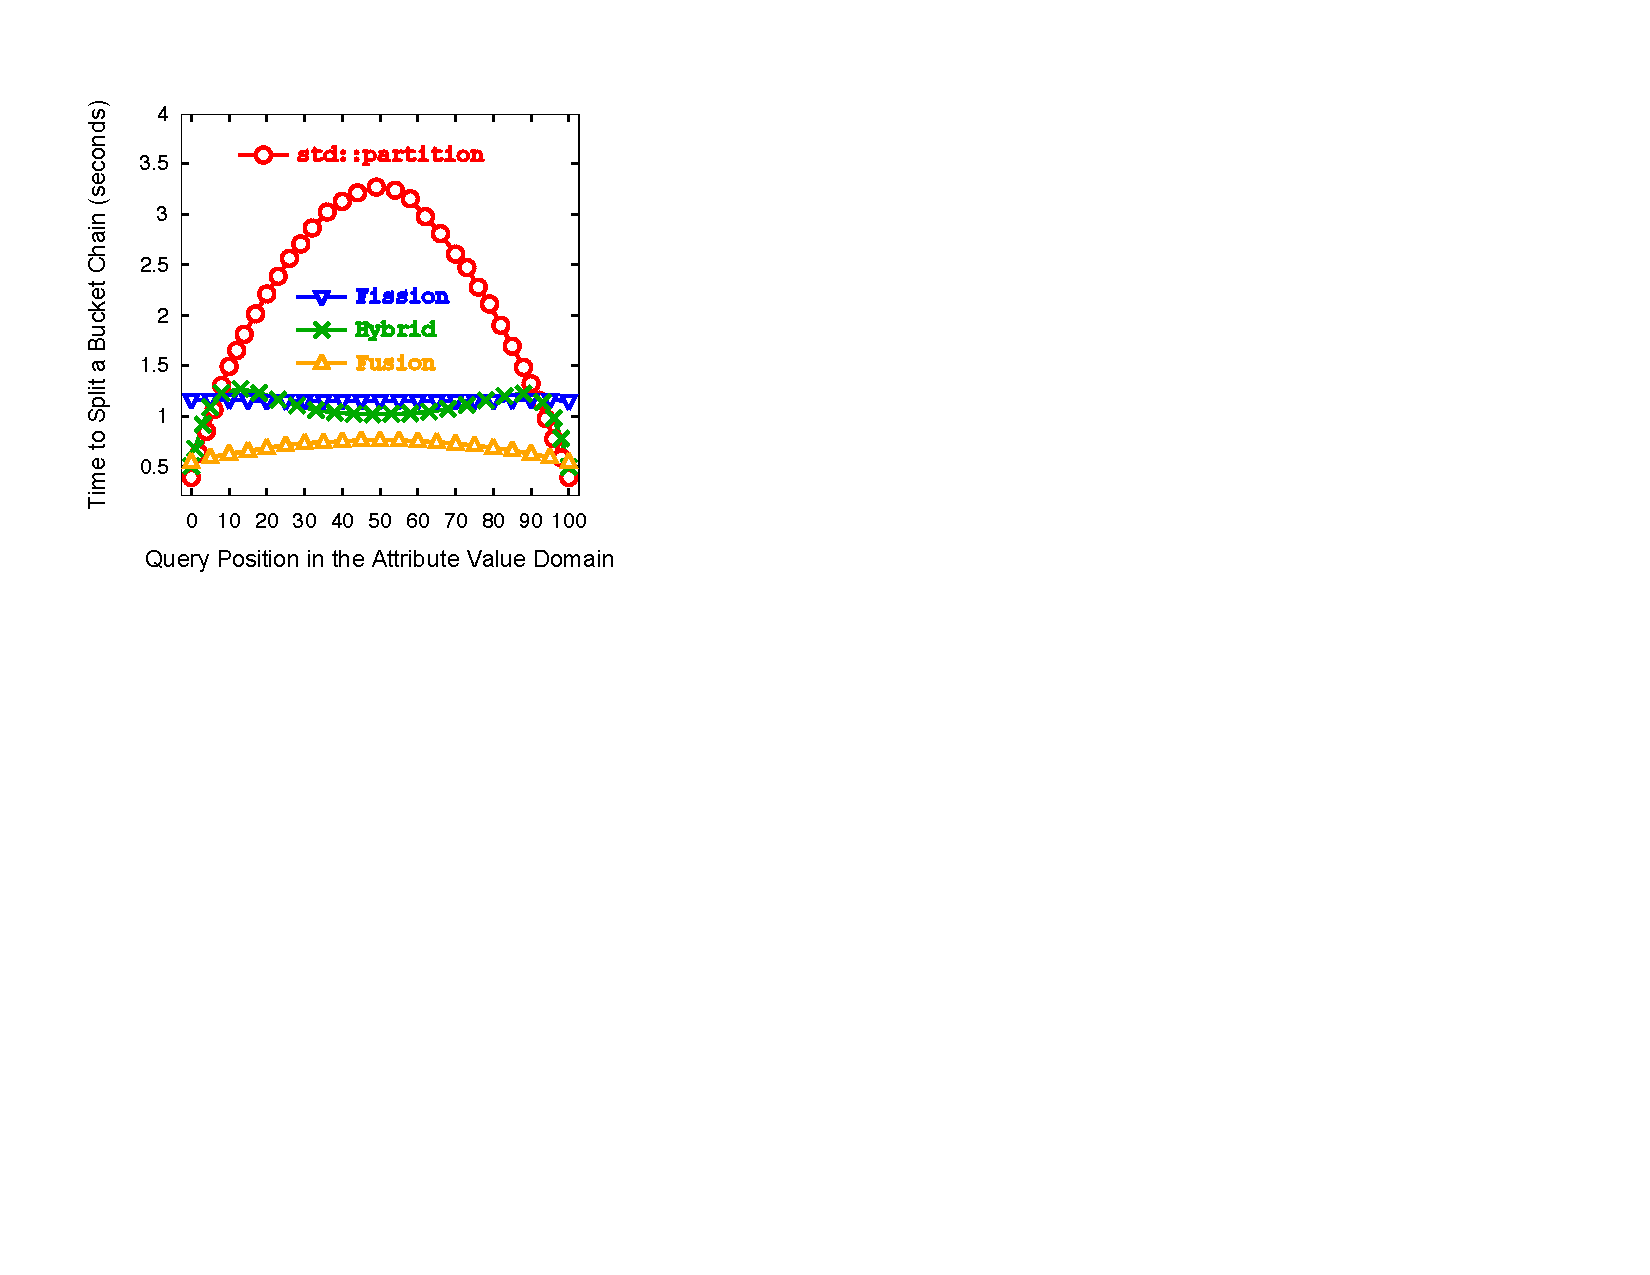
\includegraphics[width=1.055\columnwidth]{graphs/fusion.pdf}%
\vspace{-1em}
\caption{Bucket splitting.}
\vspace{-1em}
\label{F:fussion}
}
\end{figure*}

\section{Experimental Analysis}
\label{sec:experiments}

In this section, we present a detailed experimental analysis 
of Comb against state of the art adaptive indexing approaches using
both synthetic and real data sets. 
We compare Comb against original database cracking as well as against the latest 
evolutions of adaptive indexing namely stochastic database cracking \cite{StochasticCracking}, adaptive merging \cite{GK10b} 
and hybrid adaptive indexing \cite{AdaptiveIndexing}.
In addition, we compare Comb against the full indexing approach of fully sorting a column
as well as an in-memory B-tree index.
We demonstrate that Comb brings significant benefits outperforming these approaches
often by several orders of magnitude in long string of queries and updates. 


\newpage

\textbf{Resilient Adaptive Indexing.}
In our first experiment, we test Comb against original cracking in:
(i) a static many-queries scenario; and (ii) a scenario where many queries are interleaved by many updates.
The set up is the same as in the experiments of Section \ref{sec:problem}. 
The data consists of $10^8$ tuples of unique integers in $[0,2^{31})$.
The query workload is random; the ranges requested have a fixed selectivity of 1\% per query
but the actual bounds requested are random.
In the case of updates, 10 random inserts and 10 random deletes arrive every 10 read queries.

Figure \ref{F:BasicPerQueryComb} shows the results. 
In both the read only and in the updates scenario, Comb brings a significant advantage
and successfully handles the non-resilience problem of existing adaptive indexing. 
In the read only scenario in Figure \ref{F:BasicPerQueryComb}(a), 
Comb handles one billion queries in roughly fifteen minutes, while original database cracking
needs more than one hour. For the read scenario we also compare against the full indexing approach of sorting the 
column a priori. Comb is two times faster than full indexing in terms of total costs.
By carefully splitting the column in small pieces, and by keeping the buckets 
well balanced as well as 
by continuously refining the indexing information inside buckets, while adapting to the workload, Comb manages to be 
both lightweight and resilient in the long term.
Figure \ref{F:BasicPerQueryComb}(b) depicts the same results as Figure \ref{F:BasicPerQueryComb}(a) using 
logarithmic scales to more easily observe the early part of the query sequence.
Comb maintains the lightweight character of database cracking being ten times faster than the full indexing approach,
allowing for quick adaptation to the workload.
In addition, Comb starts materializing a benefit over cracking very early in the query sequence 
and in the end it is also roughly two times faster than the full indexing approach.

Figure \ref{F:BasicPerQueryComb}(c) depicts the update scenario; Comb manages to handle one billion queries in less than
one hour, while at the same time frame cracking only manages to answer 1000 times less queries, i.e., less than 1 million. 
Here, we do not include results with the full indexing approach as updating
a fully sorted column so often (every ten queries in this experiment), 
while still maintaining the dense structure of columns is prohibitively expensive.

Overall, Comb maintains both the lightweight and the adaptive character of cracking, while
bringing the resilience property, allowing to handle long strings of exploratory workloads
of continuous queries and updates.



\textbf{Comb on Real Workloads.}
For our next experiment, we demonstrate the benefits of Comb on
the SkyServer workload \cite{SkyServer}. SkyServer contains data from the astronomy domain 
and provides public database access to individual users and institutions.
We used an instance of the 4 Terabyte SkyServer data set and used $16*10^4$ queries from the query logs.
To focus on the adaptive indexing effect, i.e., within the select operator,
we filtered the selection predicates from queries.
Figure \ref{F:Skyserver} depicts the results for a sequence 
of queries using the ``right ascension" attribute of the ``Photoobjall" table.
The queries study a specific area of the sky
before moving on to a different area.
The Photoobjall table contains more than 500 million tuples, and it is one of the most commonly used ones in SkyServer. 
Data arrive continuously;
initially, only 10 million tuples are inserted. Then, every $10^3$ queries, 10 million more tuples arrive, reaching a total
of 500 million tuples by Query $5*10^4$; then another $10^4$ read only queries arrive.

Figure \ref{F:Skyserver} shows the results of comparing Comb against the state of the art 
stochastic cracking approach which was shown to be robust and more effective than plain cracking in \cite{StochasticCracking}. 
As soon as the update sequence begins, Comb materializes a significant benefit by being able to contain the update costs locally within its buckets with a small amount of data movements, 
while still being able to answer queries adaptively and efficiently.
In the end, Comb answers all queries in 1 minute, while stochastic cracking needs more than 16 hours.


\begin{figure*}[t]
\hspace{-1em}%
\Fig[b]{.95\columnwidth}{%
\hspace{1em}%
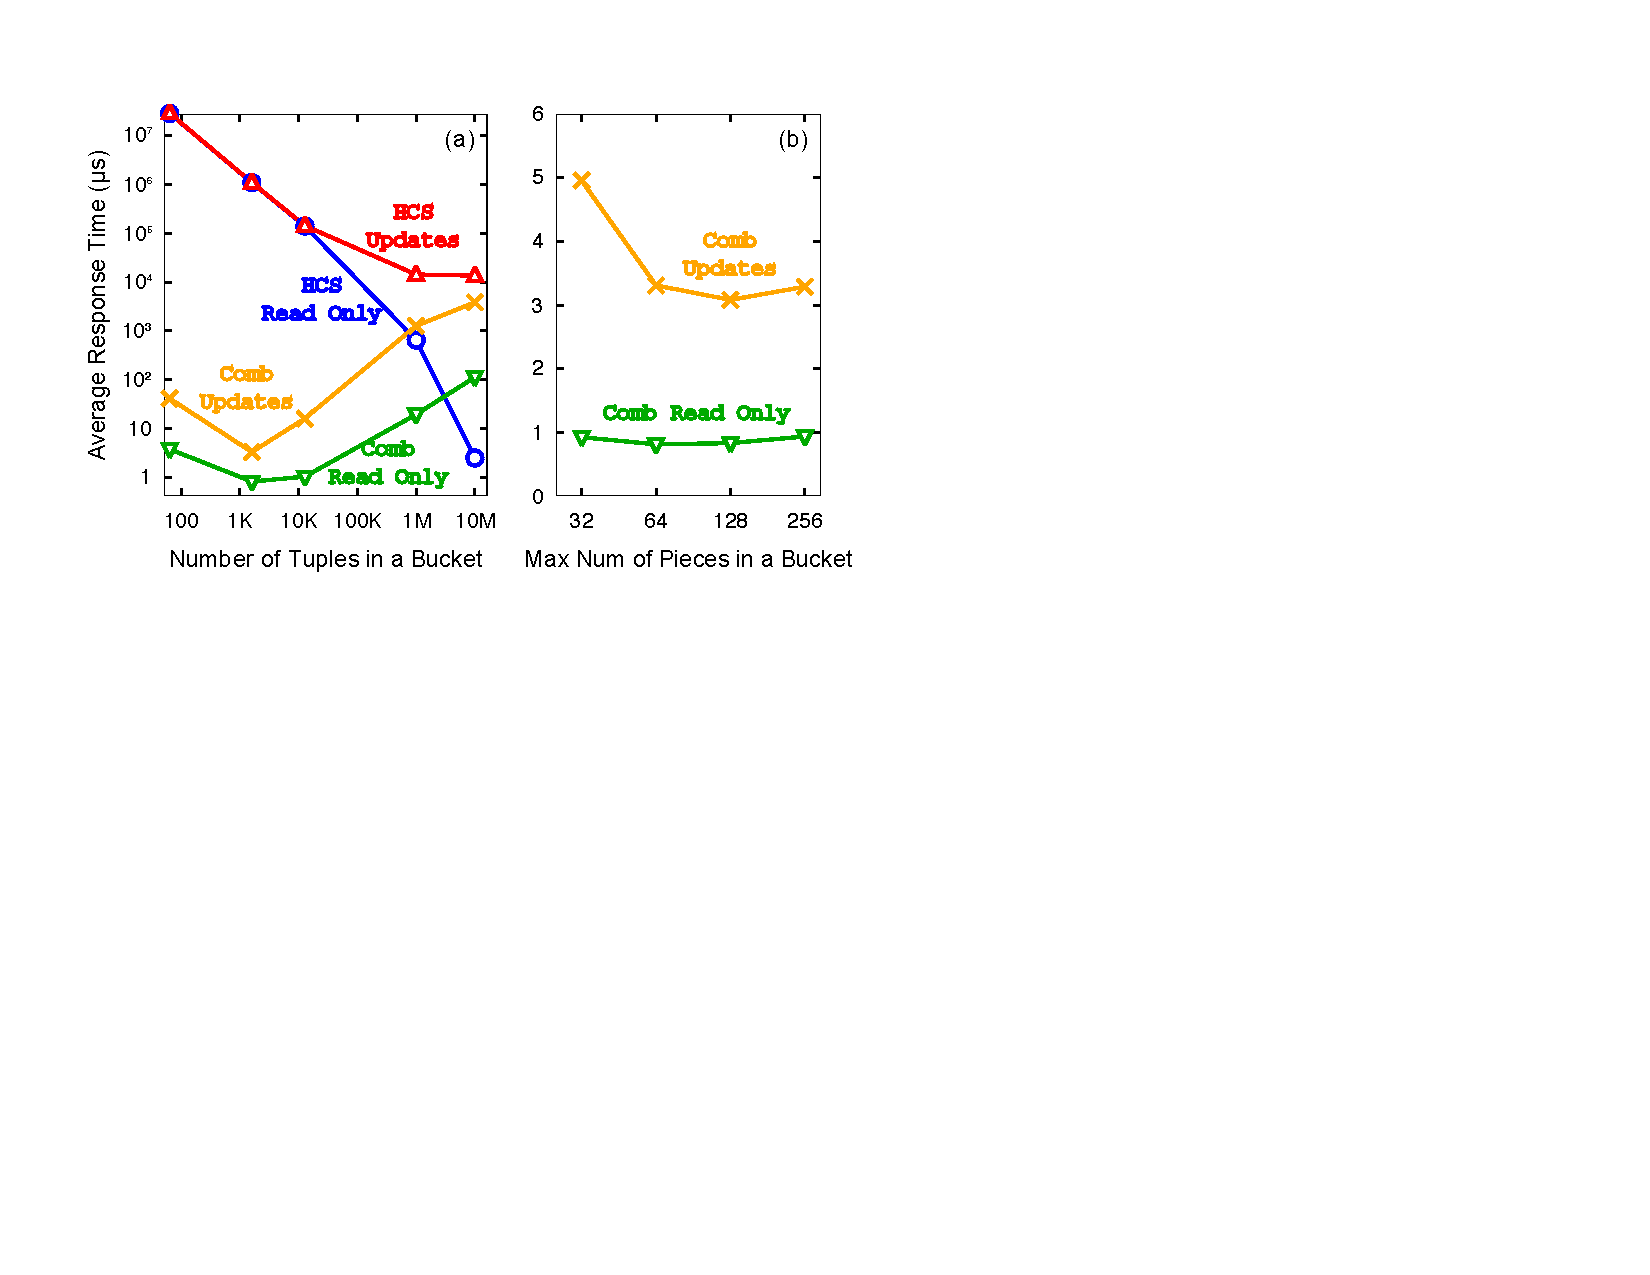
\includegraphics[width=.82\columnwidth]{graphs/hcs_comb.pdf}%
\vspace{-1em}
\caption{Varying bucket size and partitioning depth.}
\vspace{-1em}
\label{F:VaryBucketsPieces}
}
\hfill
\Fig[b]{.65\columnwidth}{%
\hspace{-3.7em}%
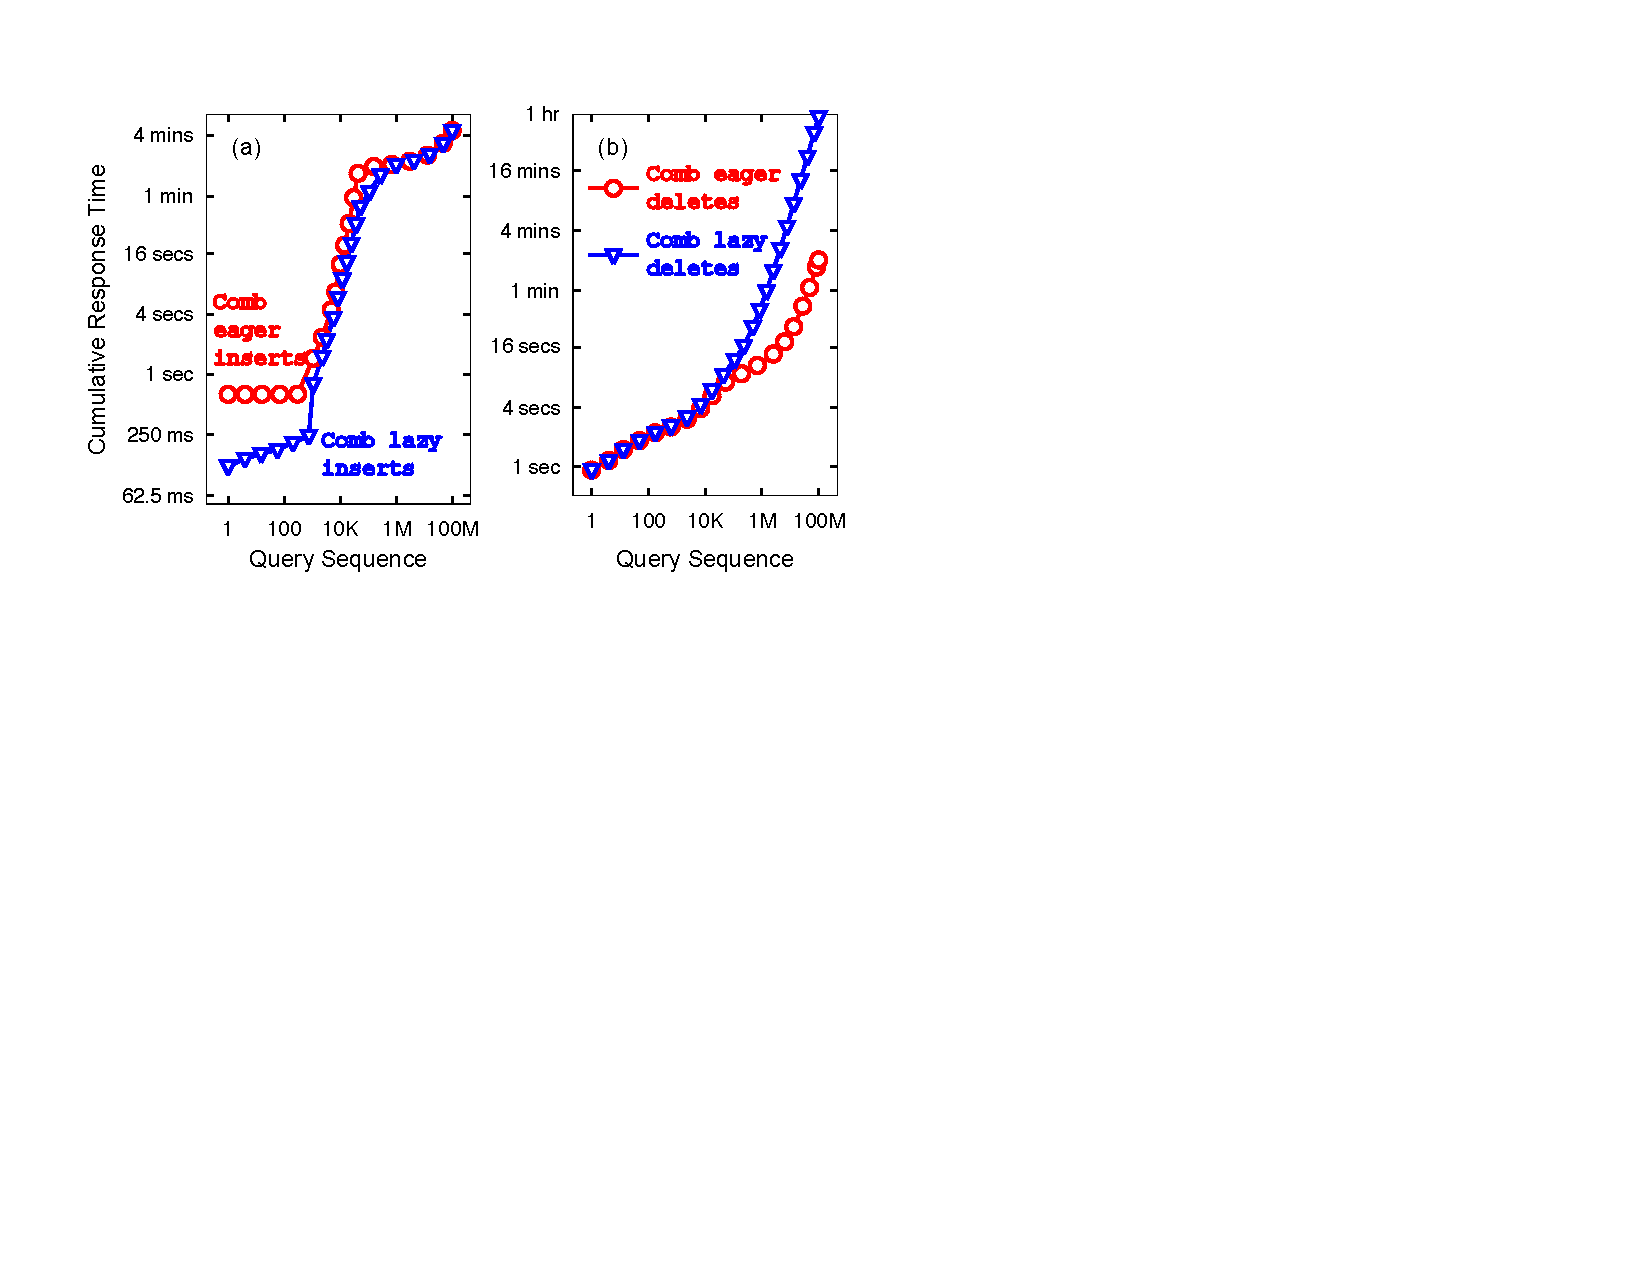
\includegraphics[width=1.2\columnwidth]{graphs/eager_lazy.pdf}%
\vspace{-1em}
\caption{Lazy V.s eager deletes/inserts.}
\vspace{-1em}
\label{F:LazyEager}
}
\hfill
\Fig[b]{.45\columnwidth}{%
\hspace{-.7em}%
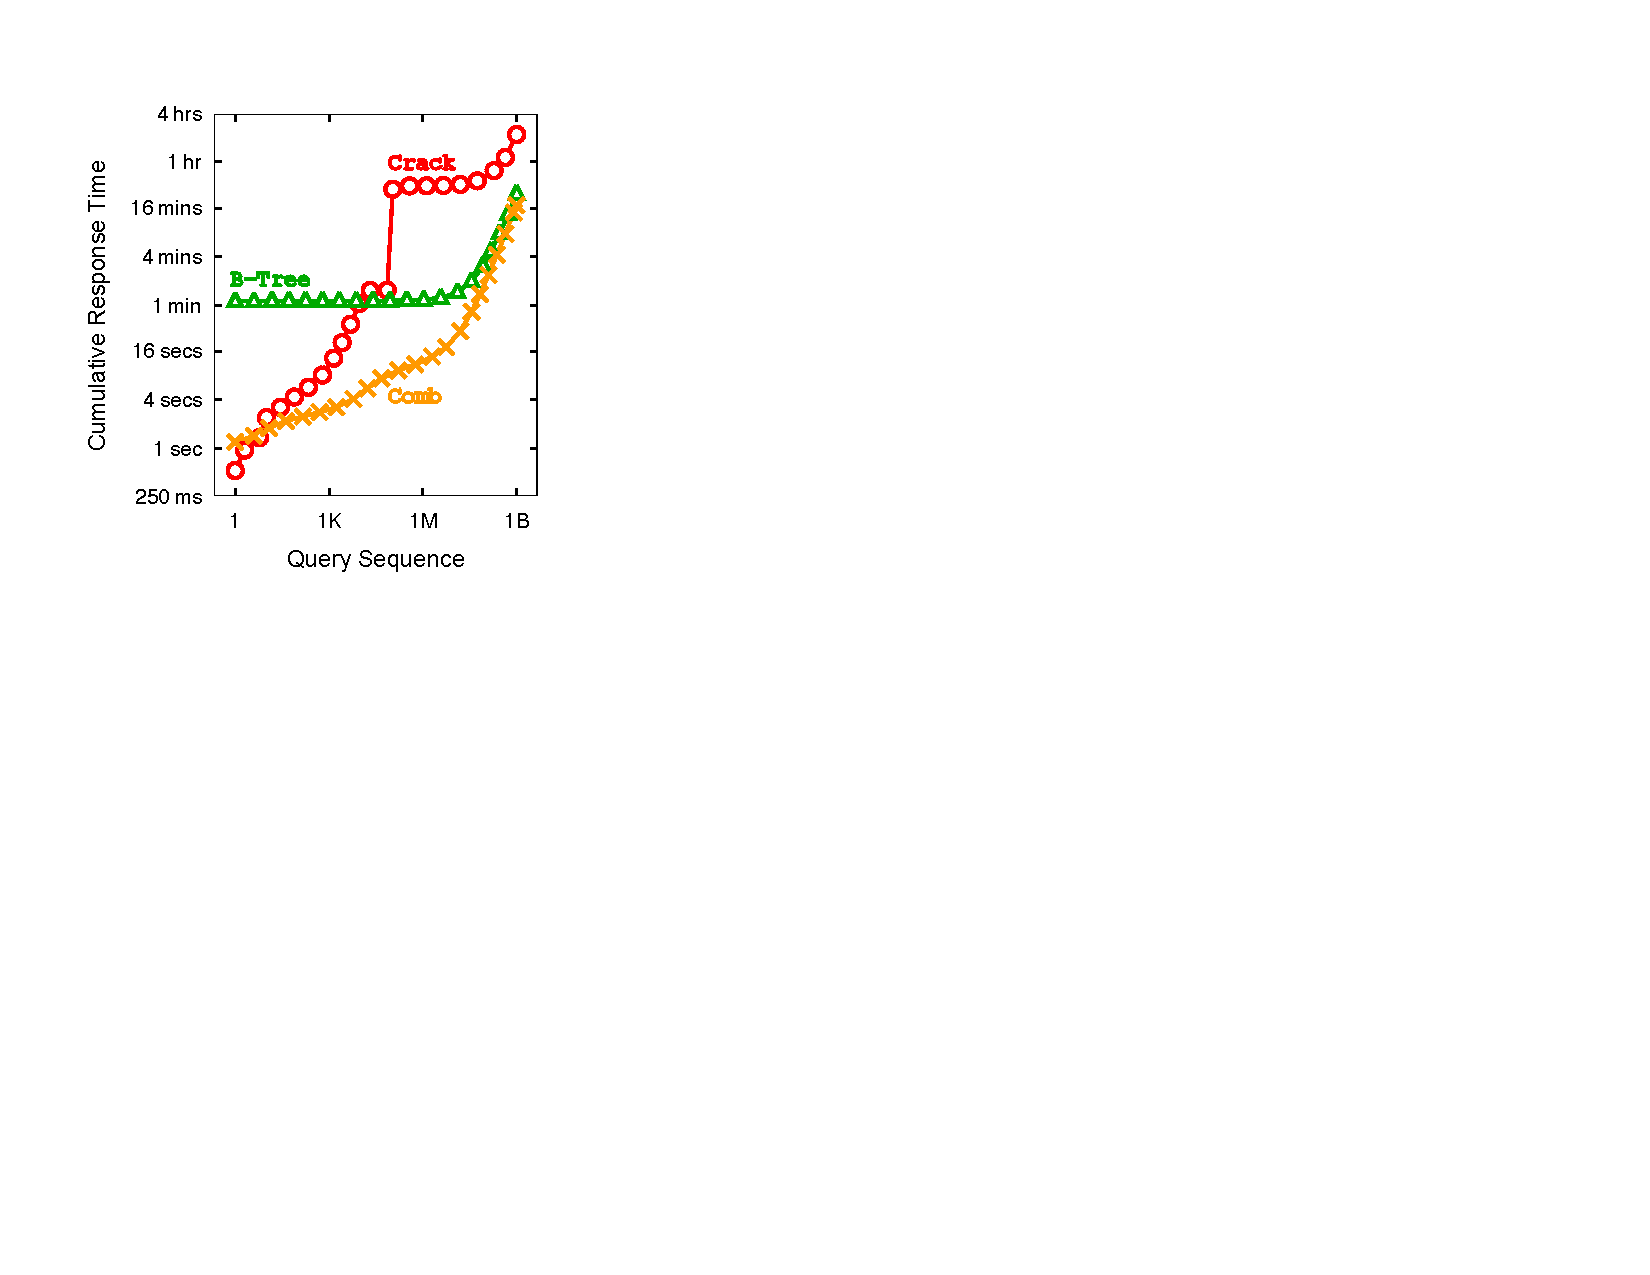
\includegraphics[width=1.06\columnwidth]{graphs/btree.pdf}%
\vspace{-1em}
\caption{Against B-tree.}
\vspace{-1em}
\label{F:Btree}
}
\end{figure*}


\textbf{Efficient Bucket Splitting.}
Splitting buckets adaptively during query processing is one of the most essential parts and cost components in Comb.
In this experiment, we demonstrate that expanding a standard partitioning algorithm is far from the optimal choice for splitting 
Comb buckets.
Figure \ref{F:fussion} demonstrates this effect. 
It shows the cost to split a chain of buckets in a Comb index. 
The chain consists of 512*256 buckets and each bucket contains 4*1024 tuples.
The $y$-axis depicts the cost to split all buckets in the chain, while varying the value of the pivot used for the splitting.
At the edges of the value domain, the pivot chosen splits a buckets in one small and one big piece, while in the 
middle of the value domain it splits the bucket in roughly two equal pieces.
Figure \ref{F:fussion} shows that when the pivot is chosen such that it splits buckets in half, the 
performance of the standard partitioning algorithm is quite poor compared to when a pivot is chosen 
at the edges of the domain. In the case of bucket splitting in Comb, we are especially interested in splitting buckets
in half such as  splitting can be effective and such that a query does less work (queries recursively split
bucket chains until they fall within a single bucket).

The reason for the poorer performance of the standard partitioning algorithm is that creating two 
equal partitions causes a significant number of branch mispredictions.
That is because the branches will fail half of the times not making it easy to predict.
Figure \ref{F:fussion} shows that our more lean chain splitting algorithm, Fission, does significantly better
by avoiding branches completely. 
Only at the very edges of the domain, standard partitioning outperforms the Fission alternative; 
then, there is no misprediction problem as all or or most branches take the same route.
Using an initial sampling phase, we are able to create a hybrid of the two approaches
where depending on the value range and the pivot we may choose the proper algorithm.
Figure \ref{F:fussion} shows that the hybrid version manages to keep the good properties of both standard partitioning and Fission.

Finally, Figure \ref{F:fussion} also depicts the behavior of the Fusion algorithm.
Fusion outperforms all other algorithms across the whole value domain.
Its strength comes from the fact that it combines the best properties from the previous variations.
It works without any branches for its core operations (as the Fission algorithm), 
while at the same time it minimizes data movements 
by doing a two pass process where it can first figure out which tuple should go where
and only then it starts moving tuples to their new location.   

 

\textbf{Effect of Bucket Size.}
Buckets are the fundamental block of Comb. 
By splitting the tuples across several buckets, Comb manages to 
handle updates and read accesses at a local per bucket level, improving 
data access patterns and minimizing data movements.
In this experiment, we study how the size of buckets may affect the performance of Comb.
As in our first experiment, the data consists of $10^8$ tuples of unique integers and queries
are chosen randomly and with a small selectivity 0.0001\%
(other selectivity factors are discussed later on). 
In the case of updates, 10 random inserts and 10 random deletes arrive every 10 queries.

Figure \ref{F:VaryBucketsPieces}(a) shows the results for both a read only scenario as well as for
a scenario where queries interleave with updates.
In both cases, a bucket size in the order of 1000-2000 tuples (in the case of 4 byte integers)
provides the best overall performance. This is a size where a bucket comfortably fits in L1 Cache.
A smaller size creates auxiliary administrative costs without bringing any more access benefits, while
a bigger size reduces administrative overheads but increases access and update costs.

Figure \ref{F:VaryBucketsPieces}(a) also depicts the performance of the state of the art hybrid adaptive 
algorithm HCS (hybrid crack-sort) which similarly to Comb also uses several buckets to store
tuples as opposed to a single column. Comb materializes a significant benefit especially when it comes 
to updates. HCS uses buckets which have overlapping value ranges and needs to physically move/merge data
to a second collection of buckets as queries arrive. On the contrary, Comb performs most of its 
index refinement actions in-place and continuously maintains buckets on non-overlapping value ranges
for the hot workload set. 
We also performed this experiment using adaptive merging (HSS \cite{AdaptiveIndexing}) which
resulted in similar performance to HCS; the only difference is that HCS is more lightweight
early in the query sequence. In the long run, performance degrades in the same way for both HCS and HSS. 



\textbf{Effect of Partitioning Depth.}
In order to reduce the excess administration and update costs, Comb puts a threshold on how deeply we can 
crack a given bucket, i.e., how many pieces we can create per bucket.
Figure \ref{F:VaryBucketsPieces}(b) shows the results of an experiment which studies the effect of 
how small or big this piece threshold should be.
The set-up is the same as in the previous experiment.
Given the small size of the bucket (set at default size of 1600 tuples) 
the number of pieces created do not significantly affect 
read only queries. In the case of updates though, there is a sweet point between 64 and 256 pieces
where both update and read costs are well balanced. The more pieces, the easier it is to locate 
a given range of tuples during a read query. On the other hand, more pieces force significant data movements
during updates. 
Comb uses 128 pieces per bucket as a default setting. 

\textbf{Eager Vs. Lazy Inserts.}
The default behavior of Comb is to chain buckets and adaptively split buckets 
during query processing and only for the ranges queried. 
This allows for an overall more lightweight behavior and an easy absorption of insertions.
In this experiment, we demonstrate the effect of a more eager strategy -- it
immediately splits buckets to place new tuples and balances the whole Comb structure during inserts.
The set-up is the same as in the previous experiment.
Figure \ref{F:LazyEager}(a) shows that overall the performance of the two approaches is rather similar in the long
run, while early in the query and update sequence the more lazy strategy allows for a more lightweight
and quick adaptation to the workload which is one of the main motivations of adaptive indexing.

\textbf{Eager Vs. Lazy Deletes.}
As we discussed in Section \ref{sec:cracke}, Comb uses a default strategy where deletes are eagerly merged
in buckets. This choice is to guarantee robustness.
Our next experiment demonstrates this behavior. 
Using a similar set-up as the previous experiments we fire a long  sequence of queries and deletes;
every 10 read queries we get 10 deletes.
Figure \ref{F:LazyEager}(b) compares the behavior of eager versus lazy deletes in Comb. 
As the sequence evolves eager deletes materialize a significant benefit;
Comb can answer 100M queries in less than 4 minutes, while with lazy deletes it needs more than 1 hour.
The main disadvantage of the lazy deletes comes from the fact that we need to check all buckets
that qualify for a range query and merge the qualifying pending deletes. This puts a significant overhead at query time. 

In the case of insertions, where Comb does use lazy inserts as a default strategy, Comb does not have to do any significant
actions during query processing. That is because inserts are placed already in the proper bucket;
they are simply out of place in terms of their local organization within the bucket.
So in a range query such as the one showed in Figure \ref{F:rangequery}, Comb only needs
to do merging actions for pending inserts for the two bound buckets at the edges of the qualifying value range. 
All buckets in between qualify but no action needs to be taken as we know that all data qualifies anyway.






\textbf{Comparison with B-tree.}
In our next experiment, we compare against a modern in-memory B-tree\footnote{\small We use the STX B+ Tree v0.8.6 (http://idlebox.net/2007/stx-btree/).} 
in a scenario where updates happen in big batches but more rarely than in previous experiments.
Using a column of $10^8$ tuples as before, this time we fire $10^6$ random inserts
just before Query 10 and another  $10^6$ random inserts just before Query $10^5$.
With original cracking, the inserts cause future queries to degrade in performance 
as they try to merge inserts in. The B-tree can handle the insertions in a graceful way
but it has a high initialization cost. 
Comb shows the same stability as the B-tree and the same lightweight adaptation as the
initial part of the cracking curve, combining the best of both worlds.  




\begin{figure}[t]
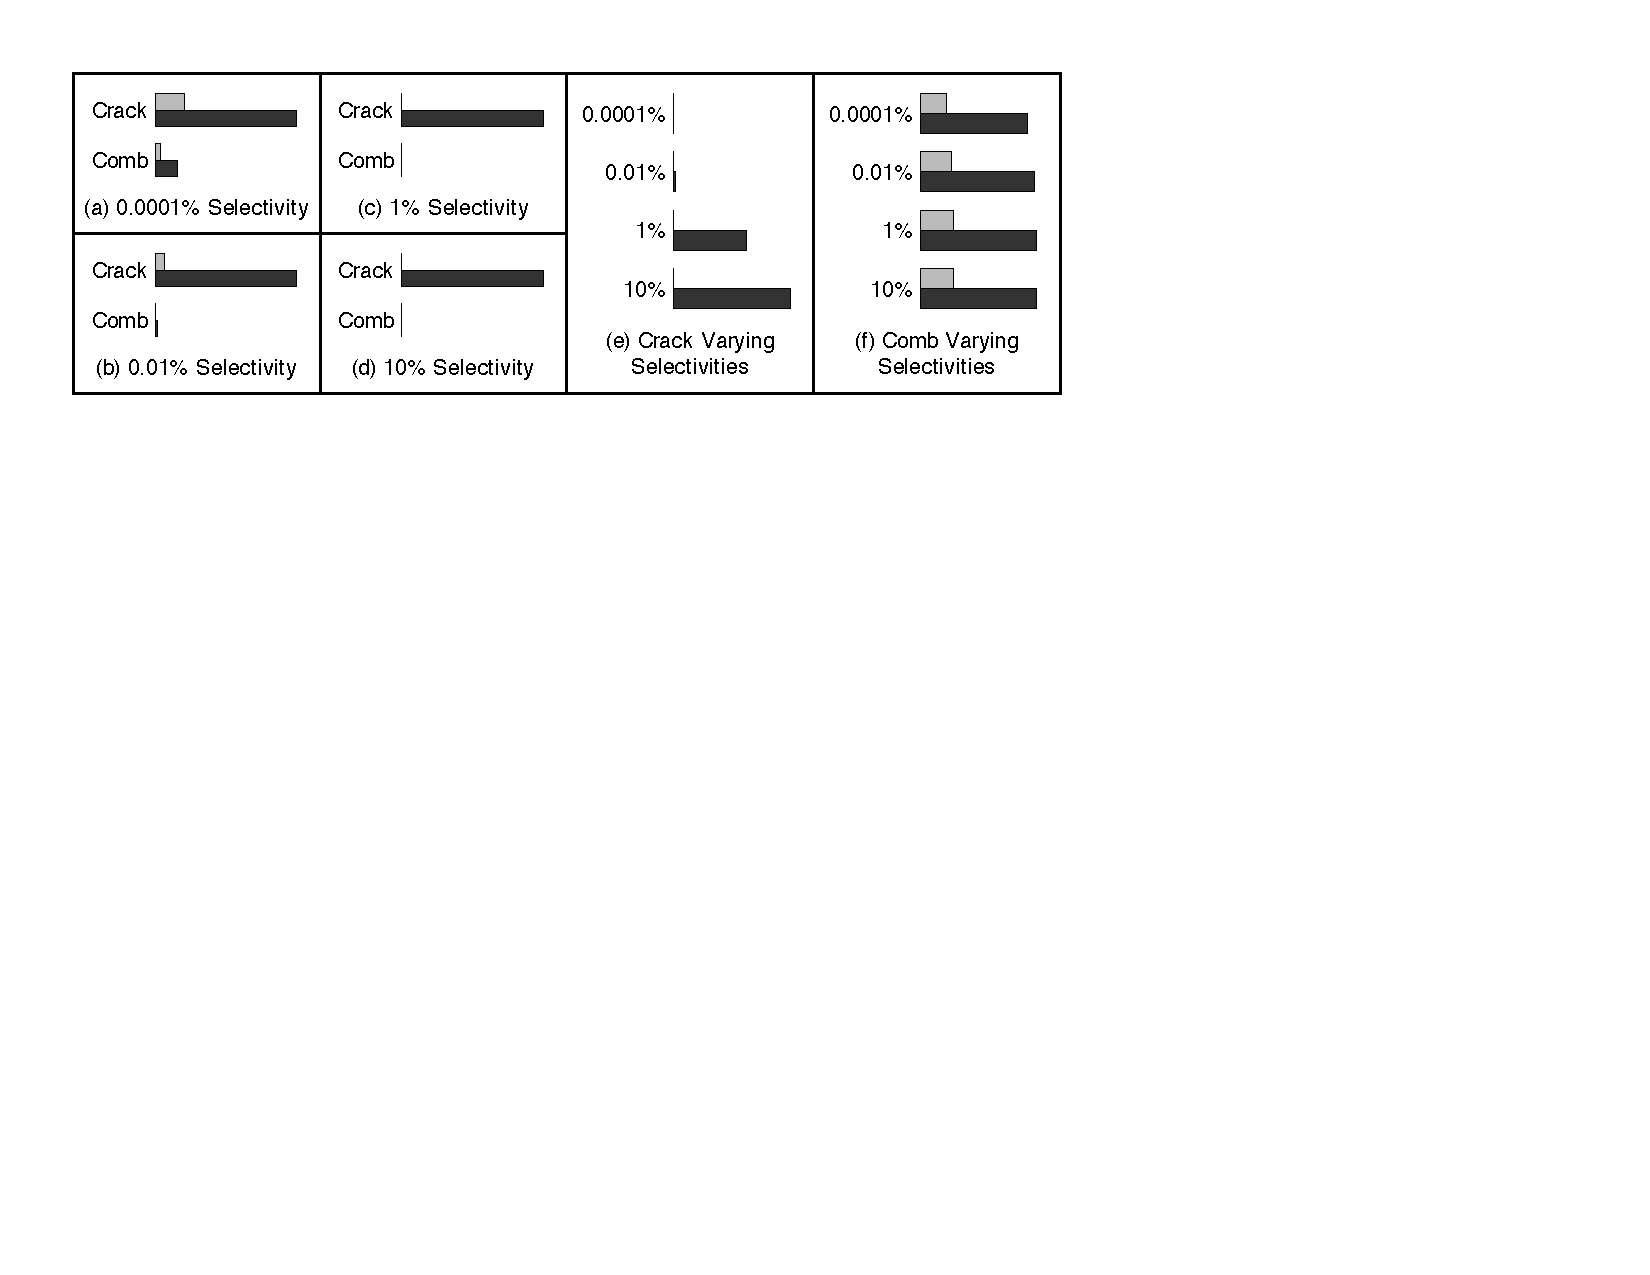
\includegraphics[width=\columnwidth]{graphs/selectivities.pdf}%
\vspace{-1em}%
\caption{Varying selectivity.}
\vspace{-2em}%
\label{F:Selectivity}
\end{figure}

\textbf{Varying Selectivity.}
In our next experiment, we demonstrate the effect of varying selectivity.
The set-up is the same as in our first experiment  with the difference that we vary the selectivity in queries.
Figure \ref{F:Selectivity} shows the results.
Figures \ref{F:Selectivity}(a)-(d) show the results for various selectivity factors.
In each box, the bars indicate normalized average query response time
with grey bars for read-only workloads and black bars when
updates interleave with queries.\footnote{
\small
We caution that normalization means that different boxes cannot be compared
as the normalization factor varies.
}
The result shows that Comb has a significant advantage across all selectivity factors.
Then, Figure \ref{F:Selectivity}(e) shows that as we vary selectivity database cracking shows a non-resilient performance
for the update workloads. What happens is that as we select bigger value ranges and thus more tuples, 
more pending updates need to be merged causing excessive update costs.
Comb on the other hand does not suffer. 
Figure \ref{F:Selectivity}(f) shows that the performance of 
Comb is stable across all selectivity factors providing a resilient and  reliable performance. 

\textbf{Optimizing Existing Adaptive Indexing.}
In our final experiment, we demonstrate that simple solutions to patch existing adaptive indexing
solutions cannot achieve the same performance as Comb which is designed from scratch for
long exploratory sequences of queries and updates.
Figure \ref{F:SimpleApproaches} shows the behavior of Comb against the 4 approaches described in Section \ref{sec:simple}.

Figures \ref{F:SimpleApproaches}(a), (b) and (c) compare Comb against the Crack-Scan, Crack-NoIndex and Crack-Sort approaches.
The experiment also varies the amount of tuples we allow inside a cracking piece in the cracker index before we choose to switch 
to the scan, sort or no-index strategy for each approach. 
As in the previous experiment, each box gives the normalized query response time
with grey bars for read-only performance
and black bars when updates interleave with queries.
Crack-Scan and Crack-NoIndex do manage to improve over plain cracking especially as the piece size threshold
becomes smaller (resulting in more pieces overall). Crack-Sort brings an extra overhead due to the expensive sorting step. 
In all cases, though, Comb manages to significantly outperform all approaches	being always 3-4 times faster than 
the second fastest approach.  


\begin{figure}[t]
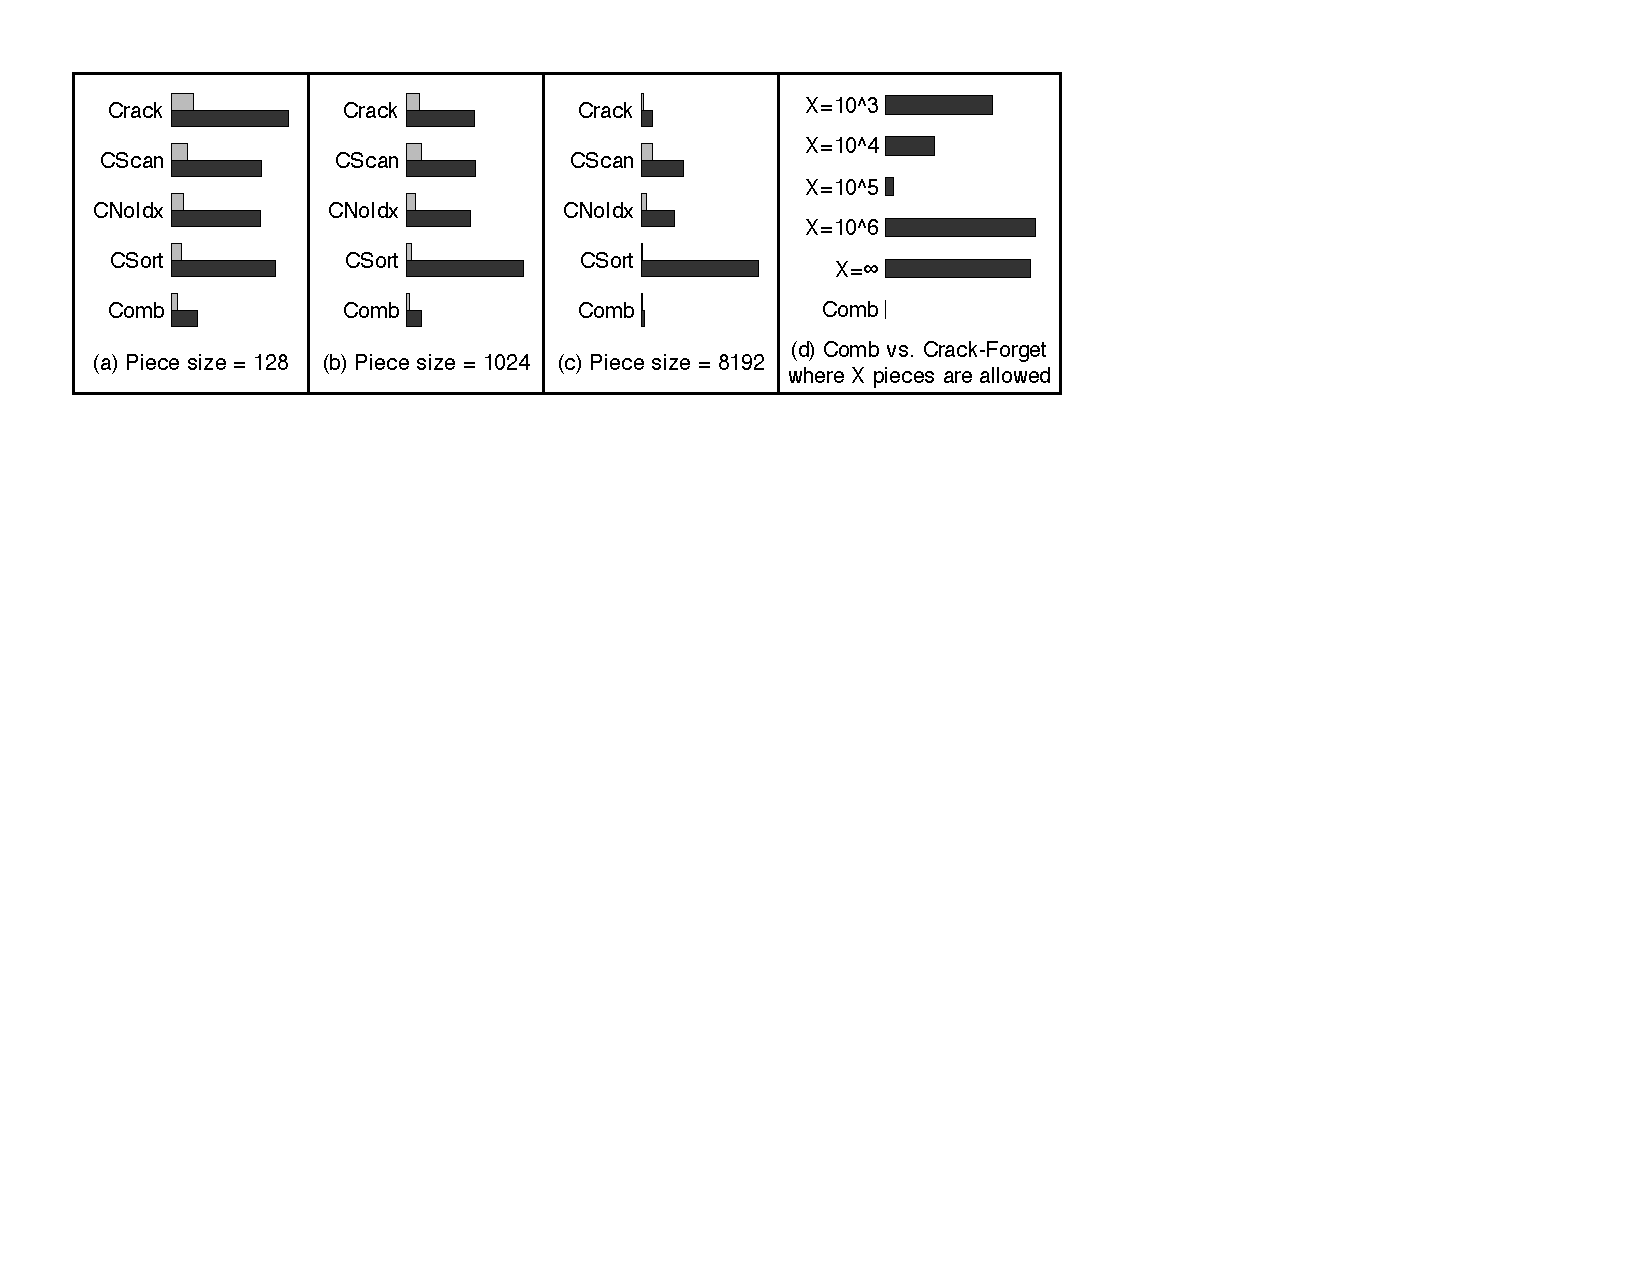
\includegraphics[width=\columnwidth]{graphs/fig_simple_w_crake.pdf}%
\vspace{-1em}%
\caption{Optimizing existing adaptive indexing.}
\vspace{-1em}%
\label{F:SimpleApproaches}
\end{figure}

Figure \ref{F:SimpleApproaches}(d) shows the performance of Comb against the Crack-Forget approach
which extends original database cracking with the ability to adaptively remove indexes
when it realizes that it needs to do expensive update actions.
It limits how many pieces it can have in the cracker index;
if the number of pieces is beyond this threshold, then  pieces which are about to be updated
are adaptively removed during query processing and thus the merging actions for updates become much more lightweight.
Figure \ref{F:SimpleApproaches}(d) shows the performance (normalized) while varying the piece threshold.
Even in the best case for Crack-Forget, Comb is 2 orders of magnitude faster.

Overall, Comb is able to outperform all patches in existing adaptive indexing approaches
and by being able to balance the costs across multiple buckets, while containing
administrative costs locally, it brings a significant performance advantage and is resilient.

 

%\section{Conclusions}
\label{sec:conclusion}
Modern applications require quick inspection of data as soon as they arrive and exploratory analysis is becoming more and more valuable. Up-front workload knowledge and idle time for tuning are scarce resources. In such environments, adaptive approaches to classic database problems are especially promising, i.e., being able to adapt data structures and strategies to the running workload. A number of techniques have been proposed in the context of adaptive indexing, providing continuous and incremental index creation. However, we show that the attractive properties of state-of-the-art adaptive indexing techniques are not resilient to new scenarios where systems are confronted with a continuous injection of new data and exploratory queries. As the sequence of data and queries evolves, adaptive indexing fails to maintain its adaptive properties and good performance in terms of quick data access.

This paper proposes Comb, a new adaptive indexing method specifically tailored for dynamic and continuously changing workloads. Based on building indexes over chains of malleable buckets, Comb maintains the beneficial properties of existing adaptive indexing approaches, while it is also resilient in those cases where current adaptive indexing fails, i.e., long strings of queries and updates. Experiments on synthetic and real workloads reveal a benefit of multiple orders of magnitude in response times.

The area of adaptive indexing is becoming progressively more mature over the years. Still there are significant future work directions towards database systems with adaptive indexing as a first-class citizen. External processing, exploitation of modern hardware such as flash disks and multi-cores, application of adaptive indexing ideas to modern row-store and hybrid architectures are a few of the open directions.
 




\bibliographystyle{abbrv}
%\scriptsize
\bibliography{references}

%\balancecolumns
\end{document}
